% --------------------------------------------------- %
%	Modelo para elaboração do Projeto de Graduação	  %		
%	do curso de Engenharia Elétrica - UFES			  %
%													  %
%	Adaptado do modelo de trabalho acadêmico 'abntex2'%
%	em 27/10/2016									  %
% --------------------------------------------------- %

\documentclass[
	% -- opções da classe memoir --
	12pt,				% tamanho da fonte
	openright,			% capítulos começam em pág ímpar (insere página vazia caso preciso)
	oneside,			% para impressão em recto e verso. Oposto a onesidehttps://www.overleaf.com/project/5b904f01df15d27389c3ec99
	a4paper,			% tamanho do papel. 
	% -- opções da classe abntex2 --
	chapter=TITLE,		% títulos de capítulos convertidos em letras maiúsculas
	%section=TITLE,		% títulos de seções convertidos em letras maiúsculas
	%subsection=TITLE,	% títulos de subseções convertidos em letras maiúsculas
	%subsubsection=TITLE,% títulos de subsubseções convertidos em letras maiúsculas
	% -- opções do pacote babel --
	english,			% idioma adicional para hifenização
	french,				% idioma adicional para hifenização
	spanish,			% idioma adicional para hifenização
	brazil				% o último idioma é o principal do documento
	]{abntex2}

% --------------------------------------------------- %
% 					Pacotes básicos 				  %
% --------------------------------------------------- %
%\usepackage{lmodern}			% Usa a fonte Latin Modern			
\usepackage[T1]{fontenc}		% Selecao de codigos de fonte.
\usepackage[utf8]{inputenc}		% Codificacao do documento (conversão automática dos acentos)
\usepackage{lastpage}			% Usado pela Ficha catalográfica
%\usepackage{indentfirst}		% Indenta o primeiro parágrafo de cada seção.
\usepackage{color}				% Controle das cores
%\usepackage{easyreview}         % Controle de revisões (adicionar ou destacar texto)
\usepackage{graphicx}			% Inclusão de gráficos
\usepackage[linesnumbered]{algorithm2e} % Formatação de escrita de algoritmos
\usepackage{microtype} 			% para melhorias de justificação
\usepackage[table,xcdraw]{xcolor} 
\usepackage{multirow}			% Para usar a tabela gerada no www.tablesgenerator.com
\usepackage{lscape}             % serve para inserir página no modo paisagem
\usepackage{pdflscape}          % serve para inserir página no modo paisagem
% \usepackage{subfig}
\usepackage{subfloat}
\usepackage{subcaption}
\usepackage{tikz}               % serve para desenhar diretamente no LaTeX


% >> Pacotes de citações
% Pacotes de citações
% ---
\usepackage[brazilian,hyperpageref]{backref}	 % Paginas com as citações na bibl
\usepackage[alf,abnt-etal-list=0,abnt-etal-cite=3]{abntex2cite}	% Citações padrão ABNT
%\usepackage[num]{abntex2cite}	% Citações padrão ABNT
% --- 
\usepackage{pdfpages}
%------------------------------------------------------------------ 
%Paquetes para la inclusion de diagramas de Gantt
\usepackage{pgfgantt}

% >> Configuração dos pacotes de citações
	% ---
	% Configurações do pacote backref
	% Usado sem a opção hyperpageref de backref
	\renewcommand{\backrefpagesname}{Citado na(s) página(s):~}
	% Texto padrão antes do número das páginas
	\renewcommand{\backref}{}
	% Define os textos da citação
	\renewcommand*{\backrefalt}[4]{
		\ifcase #1 %
			Nenhuma citação no texto.%
		\or
			Citado na página #2.%
		\else
			Citado #1 vezes nas páginas #2.%
		\fi}%
        
% >> Pacotes de teoremas e definições
\usepackage{amssymb}	 % qed
\usepackage{amsthm}      % Teoremas
\usepackage{thmtools}    % Front end para amsthm (\declaretheorem)
\declaretheorem[style=definition,name=Definição,parent=chapter,qed=\textemdash]{definicao}


% >>> Insere a pasta onde estão contidas as figuras <<<
\graphicspath{{images/}}

% --------------------------------------------------- %
%		Redefinição e criação de comandos 			  %
% --------------------------------------------------- %
\usepackage{url} %Incluir ulrs
\usepackage{xcolor} %para colorir texto
\usepackage{amsmath} %para usar \eqref{}
\usepackage{ulem} %tachar texto (comando \sout{}})
\usepackage{amsfonts} %adicionar NumberSets 

% >>> Comandos para aspas simples e duplas
\newcommand{\ASPASIMPLE}[1]{`#1'} %ASPAS SIMPLES
\newcommand{\ASPADUPLA}[1]{``#1''} %ASPAS DOBLES

\usepackage{soul} % para tachar palabras
\newcommand{\warning}[1]{\textcolor{magenta}{#1}}
\newcommand{\add}[1]{\textcolor{blue}{#1}}
\newcommand{\review}[1]{\textcolor{green}{#1}}
\newcommand{\remove}[1]{\textcolor{red}{\st{#1}}}
\newcommand{\passive}[1]{\textcolor{\textbf{yellow}}{\st{#1}}}
\newcommand{\wordchoice}[1]{\textcolor{\textbf{yellow}}{\st{#1}}}
\newcommand{\recom}[2]{\remove{#1} \add{#2}}
% >>> Comando para colorear texto
\newcommand{\txr}[1]{\textcolor{red}{\textbf{#1}}}
\newcommand{\txg}[1]{\textcolor{green}{\textbf{#1}}}
\newcommand{\txb}[1]{\textcolor{blue}{\textbf{#1}}}
\newcommand{\txk}[1]{\textbf{\textbf{#1}}}

% >>> Comando para vetores
\newcommand{\mat}[1]{\mbox{\boldmath{$#1$}}}
\newcommand{\aaa}{\textbf{a}}
\newcommand{\oo}{\textbf{o}}
\newcommand{\ww}{\textbf{w}}
\newcommand{\xx}{\textbf{x}}
\newcommand{\yy}{\textbf{y}}
\newcommand{\zz}{\textbf{z}}
\newcommand{\THETA}{\mat{\theta}}

%%%%%%%%%%%%%%%%%%%%%%%%%%%%%%%%%%%%%%%%%%%%%%%%%%%%%
%%%%%%%%%%%%%%%%%%%%%%%%%%%%%%%%%%%%%%%%%%%%%%%%%%%%%
%%%%%%%%%%%%%%%%%%%%%%%%%%%%%%%%%%%%%%%%%%%%%%%%%%%%%
%variavel que permite trocar entre o modelo de PG (para PG 1) e TCC (para PG 2)
%por default esta em PG
\newif\ifisTipoDocumento
\newif\ifisFolhaAprovacao
\isTipoDocumentotrue %PG (descomentar em caso de PG 1)
%\isTipoDocumentofalse %TCC (descomentar em caso de PG 2)
%\isFolhaAprovacaotrue %TCC (PG 2) finalizado
%\isFolhaAprovacaofalse %TCC (PG 2) não finalizado

%%%%%%%%%%%%%%%%%%%%%%%%%%%%%%%%%%%%%%%%%%%%%%%%%%%%%
%%%%%%%%%%%%%%%%%%%%%%%%%%%%%%%%%%%%%%%%%%%%%%%%%%%%%
%%%%%%%%%%%%%%%%%%%%%%%%%%%%%%%%%%%%%%%%%%%%%%%%%%%%%

% >>> Mudar tamanho da fonte dos capítulos <<<
\renewcommand*{\chapnumfont}{\normalfont\large\bfseries\sffamily}
\renewcommand*{\chaptitlefont}{\normalfont\large\bfseries\sffamily}

\usepackage{titlesec}
\titleformat{\section}
  {\normalfont\normalsize\bfseries}{\thesection}{1em}{}
\titleformat{\subsection}
  {\normalfont\normalsize\bfseries}{\thesubsection}{1em}{}

% >>> Mudar tamanho da fonte das legendas <<<
\usepackage[font=footnotesize]{caption}

% >>> Definição do tipo CRONOGRAMA <<<
% e.g.:
% \begin{cronograma}[!h]
% 		Insira o cronograma aqui! (tabela)
% \eng{cronograma}
\newcommand{\cronogramaname}{Cronograma}
\newcommand{\listofcronogramasname}{Lista de Cronogramas}

\newfloat[chapter]{cronograma}{loc}{\cronogramaname}
\newlistof{listofcronogramas}{loc}{\listofcronogramasname}
\newlistentry{cronograma}{loc}{0}

\counterwithout{cronograma}{chapter}
\renewcommand{\cftcronogramaname}{\cronogramaname\space} 
\renewcommand*{\cftcronogramaaftersnum}{\hfill--\hfill}

% >>> Definição do tipo QUADRO <<<
% e.g.:
% \begin{quadro}[!h]
%  Insira aqui o quadro (tabela)
% \end{quadro} 
\newcommand{\quadroname}{Quadro}
\newcommand{\listofquadrosname}{Lista de Quadros}

\newfloat[chapter]{quadro}{loq}{\quadroname}
\newlistof{listofquadros}{loq}{\listofquadrosname}
\newlistentry{quadro}{loq}{0}

\counterwithout{quadro}{chapter}
\renewcommand{\cftquadroname}{\quadroname\space} 
\renewcommand*{\cftquadroaftersnum}{\hfill--\hfill}

% >>> Comando para inserir a fonte em figuras <<<
% e.g.:
% \begin{figure}[!h]
%	\centering
%	\caption{Legenda da Figura.}
%	\includegraphics[width=0.7\textwidth]{figura.jpg}
%	\source[\citeonline{Referencia}.]
%	\label{fig:label_da_figura}
%  \end{figure}
%  
% Obs.: Se utilizar apenas "\source", será inserido
%       "Produção do próprio autor."

\newcommand{\source}[1][Produção do próprio autor.]{\begin{flushleft}\footnotesize Fonte: #1\end{flushleft}}

% --------------------------------------------------- %
%		    Dados do autor/banca/data	      	  	  %	
% --------------------------------------------------- %
\newcommand{\TituloDoTCC}{\uppercase{Uma proposta de expansão de um Espaço Inteligente Programável através de dispositivos robóticos e computação em borda}}
\newcommand{\NomeDeAutor}{Luiz Carlos Cosmi Filho}
\newcommand{\NomeOrientador}{Profa. Dra. Raquel Frizera Vassallo}
\newcommand{\NomeCoorientador}{Prof. Dr. Alexandre Pereira do Carmo}
\newcommand{\DataApresentacao}{Dezembro/2023}

% --------------------------------------------------- %
%		Informações para personalização da capa		  %
% --------------------------------------------------- %
\newcommand{\universidade}{Universidade Federal do Espírito Santo}
\newcommand{\centro}{Centro Tecnológico}
\newcommand{\departamento}{Departamento de Engenharia Elétrica}
\newcommand{\disciplina}{Projeto de Graduação}
\newcommand{\imprimirINSTITUICAO}{
	\MakeUppercase{\universidade} \\
	\MakeUppercase{\centro} \\
	\MakeUppercase{\departamento} \\
	\MakeUppercase{\disciplina} \\
}
% --------------------------------------------------- %
%		Informações para capa e folha de rosto		  %
% --------------------------------------------------- %
\titulo{\TituloDoTCC}
\autor{\NomeDeAutor}
\local{Vitória-ES}
\data{\DataApresentacao}
\orientador{\NomeOrientador}
\coorientador{\NomeCoorientador}
\instituicao{%
	\universidade
  	\par
	\centro
  	\par
	\departamento
	\par
	\disciplina
	\par}
\tipotrabalho{Projeto de Graduação}
% O preambulo deve conter o tipo do trabalho, o objetivo, 
% o nome da instituição e a área de concentração 
\preambulo{Parte manuscrita do Projeto de Graduação do aluno \NomeDeAutor, apresentado ao Departamento de Engenharia Elétrica do Centro Tecnológico da Universidade Federal do Espírito Santo, como requisito parcial para obtenção do grau de Engenheiro Eletricista.}

% --------------------------------------------------- %
%		Configurações do aspecto final do PDF		  %
% --------------------------------------------------- %
% >> Alterando o aspecto da cor azul
\definecolor{blue}{RGB}{41,5,195}
% Informações do PDF
\makeatletter
\hypersetup{
     	%pagebackref=true,
		pdftitle={\@title}, 
		pdfauthor={\@author},
    	pdfsubject={\imprimirpreambulo},
	    pdfcreator={LaTeX with abnTeX2},
		pdfkeywords={abnt}{latex}{abntex}{abntex2}{trabalho acadêmico}, 
		colorlinks=true,       		% false: boxed links; true: colored links
    	linkcolor=black,          	% color of internal links
    	citecolor=black,        		% color of links to bibliography
    	filecolor=magenta,      		% color of file links
		urlcolor=black,
		bookmarksdepth=4
}
\makeatother

% --------------------------------------------------- %
%		Espaçamentos entre linhas e parágrafos 		  %
% --------------------------------------------------- %
% >> O tamanho do parágrafo é dado por:
\setlength{\parindent}{0cm}
% >> Controle do espaçamento entre um parágrafo e outro:
\setlength{\parskip}{18pt}

% --------------------------------------------------- %
%				Compila o Índice 					  %
% --------------------------------------------------- %
\makeindex

% --------------------------------------------------- %
%				Início do Documento					  %
% --------------------------------------------------- %

\begin{document}

% >>> Seleciona o idioma do documento (conforme pacotes do babel)
% \selectlanguage{english}
\selectlanguage{brazil}

% >>> Retira espaço extra obsoleto entre as frases.
\frenchspacing 

% --------------------------------------------------- %
%				Elementos Pré-Textuais				  %
% --------------------------------------------------- %
% \pretextual

%%%%%%%%
\ifisTipoDocumento
% --------------------------------------------------- %
%						Capa						  %
% --------------------------------------------------- %
% >>> Capa Personalizada
\renewcommand{\imprimircapa}{%
	\begin{capa}%
		\center
		{\ABNTEXchapterfont\bfseries\large\imprimirINSTITUICAO}
			\vspace*{1.5cm}
		\includegraphics*[width=0.25\textwidth]{brasao-ufes.jpg}
			\vspace*{1.5cm} \\
		{\ABNTEXchapterfont\bfseries\Large\MakeUppercase\imprimirautor}
				\vspace*{2.5cm} \\
		{\ABNTEXchapterfont\bfseries\Large\imprimirtitulo}
			\vfill
			\vspace*{0.5cm}
		{\large\MakeUppercase\imprimirlocal}
		\par
		{\large\MakeUppercase\imprimirdata}
			\vspace*{1cm}
	\end{capa}
}

\imprimircapa

% --------------------------------------------------- %
%					Folha de Rosto 					  %
% --------------------------------------------------- %
% >> O * indica que haverá a ficha bibliográfica

\renewcommand{\imprimirfolhaderosto}{

\begin{folhaderosto}
	\begin{center}
    	{\ABNTEXchapterfont\large\imprimirautor}
		    \vspace*{\fill}\vspace*{\fill}
    	\begin{center}
	    	\ABNTEXchapterfont\bfseries\Large\imprimirtitulo
	    \end{center}
    		\vspace*{\fill}
    		\hspace{.45\textwidth}
	    \begin{minipage}{.5\textwidth}
        	\imprimirpreambulo
	    \end{minipage}
    		\vspace*{\fill}
	    \end{center}  
        \begin{center}
        	% >> Se necessáiro, ajustar os \vspace
        	%\vspace*{0.5cm}
        {\large\imprimirlocal}
        \par
        {\large\imprimirdata}
       		%\vspace*{1cm}
      \end{center}
\end{folhaderosto}
}

\imprimirfolhaderosto

% --------------------------------------------------- %
%					Ficha Catalográfica 			  %
% --------------------------------------------------- %

% Isto é um exemplo de Ficha Catalográfica, ou ``Dados internacionais de
% catalogação-na-publicação''. Você pode utilizar este modelo como referência. 
% Porém, provavelmente a biblioteca da sua universidade lhe fornecerá um PDF
% com a ficha catalográfica definitiva após a defesa do trabalho. Quando estiver
% com o documento, salve-o como PDF no diretório do seu projeto e substitua todo
% o conteúdo de implementação deste arquivo pelo comando abaixo:
%
% \begin{fichacatalografica}
%     \includepdf{fig_ficha_catalografica.pdf}
% \end{fichacatalografica}

%\begin{fichacatalografica}
%	\sffamily
%	\vspace*{\fill}					% Posição vertical
%	\begin{center}					% Minipage Centralizado
%	\fbox{\begin{minipage}[c][8cm]{13.5cm}		% Largura
%	\small
%	\imprimirautor
%	%Sobrenome, Nome do autor
%	
%	\hspace{0.5cm} \imprimirtitulo  / \imprimirautor. --
%	\imprimirlocal, \imprimirdata-
%	
%	\hspace{0.5cm} \pageref{LastPage} p. : il. (algumas color.) ; 30 cm.\\
%	
%	\hspace{0.5cm} \imprimirorientadorRotulo~\imprimirorientador\\
%	
%	\hspace{0.5cm}
%	\parbox[t]{\textwidth}{\imprimirtipotrabalho~--~\imprimirinstituicao,
%	\imprimirdata.}\\
%	
%	\hspace{0.5cm}
%		1. Palavra-chave1.
%		2. Palavra-chave2.
%		2. Palavra-chave3.
%		I. Orientador.
%		II. Universidade xxx.
%		III. Faculdade de xxx.
%		IV. Título 			
%	\end{minipage}}
%	\end{center}
%\end{fichacatalografica}

% --------------------------------------------------- %
%					Folha de Aprovação			      %
% --------------------------------------------------- %
% >>> Após apresentação do trabalho, substitua todo o conteúdo 
% por uma imagem da página assinada pela banca com o comando abaixo:
%\includepdf{aprovacao.pdf}

 \begin{folhadeaprovacao}
   \begin{center}
     {\ABNTEXchapterfont\large\imprimirautor}
 	\begin{center}
      	\ABNTEXchapterfont\bfseries\Large\imprimirtitulo
     \end{center}
     %\vspace*{\fill}
   \end{center}    
     \imprimirpreambulo
 		\vspace{-0.5cm}
     \begin{center}
 		\hspace{.45\textwidth}
     \begin{minipage}{.5\textwidth}
%         \textbf{COMISSÃO EXAMINADORA:}
\assinatura{\textbf{Profa. Dra. Marcia Helena Moreira Paiva} \\ Universidade Federal do Espírito Santo \\ Professor da Disciplina}
\assinatura{\textbf{\imprimirorientador} \\ Universidade Federal do Espírito Santo \\ Orientadora} 
\assinatura{\textbf{\imprimircoorientador} \\ Universidade Federal do Espírito Santo \\ Coorientador}
\assinatura{\textbf{\imprimirautor} \\ Universidade Federal do Espírito Santo \\ Aluno}
% 		\assinatura{\textbf{Prof. Dr. Pedro Pedrinho} \\ Universidade Federal do Espírito Santo \\ Examinador}
% 		\assinatura{\textbf{Msc. João da Vida} \\ Universidade Federal do Espírito Santo \\ Examinador}
     \end{minipage}
 	    \vspace*{\fill}
    \end{center}
         
    \begin{center}
       	% >> Se necessáiro, ajustar os \vspace
 		%\vspace*{0.5cm}
     	{\large\imprimirlocal}
     	\par
     	{\large\imprimirdata}
    		%\vspace*{1cm}
   \end{center}  
 \end{folhadeaprovacao}
 
 
 % --------------------------------------------------- %
%						Resumo				      	  %	
% --------------------------------------------------- %

% Resumo em português
\setlength{\absparsep}{18pt} % ajusta o espaçamento dos parágrafos do resumo
\begin{resumo}

% {\sffamily This is a sample text in \textbf{Sans Serif Font Typeface}}
% Identifica qual é a grande área onde seu trabalho esta inserido e qual é a importância dessa grande área.
% \textbf{2. \txr{Gaps ou vazios}}
% Aqui o autor diz que coisa na grande área precisa ser pesquisada. 
% Aqui é onde o autor deixa claro o que ainda não esta bem entendido, esta em aberto ou é controvertido. 
% Em resumo, o Gap é o vazio dessa grande área na qual  o trabalho esta inserido. 
% O comum é iniciar con as palavras: \textit{ainda}, \textit{Sem embargo}
% \textbf{\txr{3. Proposta}}
% Em esta parte o autor indica qual é o proposta e o objetivo do trabalho, evidentemente o objetivo deve estar relacionado con el Gap. O comum é iniciar con as frases: \textit{Este trabalho descreve ...}; \textit{Este trabalho reporta ...}; \textit{Aqui, ...}; \textit{Em este trabalho, é proposto, ... }.
% \textbf{\txr{4. Metodologia}}
% Aqui são descritos os métodos utilizados para a realização do trabalho.
% \textbf{\txr{5. Resultados}}
% Esta parte do resumo é extremadamente importante, não existe resumo que não tenha seção de resultados bem clara e detalhada, cabe ao autor identificar qual é seu principal resultado, para deixar bem claro no resumo.  Acontinuação um exemplo.

% \textbf{1. \txr{Contextualização}}
% O câncer de pele é o tipo de câncer mais comum no Brasil. 
% O melanoma é seu subtipo mais mortal. 
% Portanto, é essencial que seja detectado em seus estágios iniciais, quando a taxa de sobrevivência ainda é alta. 
% Entretanto, ele é muito fácil de ser confundido por pintas comuns ou outros tipos de lesões de pele, até mesmo por especialistas. 
% \textbf{2. \txr{Gaps ou vazios}}
% Assim, alguma ferramenta de diagnóstico automatizado se torna indispensável. 
% Porém, as soluções automatizadas existentes não são muito superiores aos diagnósticos comuns. 
% A partir de $2012$ houveram grandes avanços na aplicação de redes neurais para a classificação de imagens. 
% A aplicação de redes neurais convolucionais profundas está superando a performance humana em diversas tarefas. 
% \textbf{3. \txr{Proposta}}
% O presente projeto de graduação faz uso de uma rede convolucional para tentar solucionar o problema de classificação binária de imagens de melanomas ou ceratoses seborréicas contra nevos. 
% A tarefa a solucionar foi obtida do desafio ISIC 2017, que provê um banco de dados para realizar o treino das redes e para validar a solução. 
% \textbf{4. \txr{Metodologia}}
% Para auxiliar e facilitar a tarefa foram usadas as técnicas de pré-processamento de imagens e transferência de aprendizado. 
% Um estudo aprofundado é feito sobre a arquitetura da rede usada, detalhando seu funcionamento interno. São treinados diversos classificadores para a tarefa dos quais o melhor obteve um desempenho equiparável a soluções de outras equipes. 
% \textbf{5. \txr{Resultados}}
% Especificamente, é obtido uma média de área sob a curva de característica de operação do receptor de $0.877$ quando testado no banco de dados do desafio ISIC 2017, ficando situado entre os 10 melhores resultados.

xxxxx.

\textbf{Palavras-chave}: Computação em borda; Computação em Nuvem, Espaços Inteligentes.
\end{resumo}

% --------------------------------------------------- %
%					Resumo em ingles	      	  	  %	
% --------------------------------------------------- %
\begin{resumo}[Abstract]
 \begin{otherlanguage*}{english}
   \noindent xxxxx.
   
   \textbf{Keywords}: Edge Computing; Cloud computing; Intelligent Spaces.
 \end{otherlanguage*}
\end{resumo}
\else
% --------------------------------------------------- %
%						Capa						  %
% --------------------------------------------------- %
% >>> Capa Personalizada
\renewcommand{\imprimircapa}{%
	\begin{capa}%
		\center
		{\ABNTEXchapterfont\bfseries\large\imprimirINSTITUICAO}
			\vspace*{1.5cm}
		\includegraphics*[width=0.25\textwidth]{brasao_ufes.jpg}
			\vspace*{1.5cm} \\
		{\ABNTEXchapterfont\bfseries\Large\MakeUppercase\imprimirautor}
				\vspace*{2.5cm} \\
		{\ABNTEXchapterfont\bfseries\Large\imprimirtitulo}
			\vfill
			\vspace*{0.5cm}
		{\large\MakeUppercase\imprimirlocal}
		\par
		{\large\MakeUppercase\imprimirdata}
			\vspace*{1cm}
	\end{capa}
}

\imprimircapa

% --------------------------------------------------- %
%					Folha de Rosto 					  %
% --------------------------------------------------- %
% >> O * indica que haverá a ficha bibliográfica

\renewcommand{\imprimirfolhaderosto}{

\begin{folhaderosto}
	\begin{center}
    	{\ABNTEXchapterfont\large\imprimirautor}
		    \vspace*{\fill}\vspace*{\fill}
    	\begin{center}
	    	\ABNTEXchapterfont\bfseries\Large\imprimirtitulo
	    \end{center}
    		\vspace*{\fill}
    		\hspace{.45\textwidth}
	    \begin{minipage}{.5\textwidth}
        	\imprimirpreambulo
	    \end{minipage}
    		\vspace*{\fill}
	    \end{center}  
        \begin{center}
        	% >> Se necessáiro, ajustar os \vspace
        	%\vspace*{0.5cm}
        {\large\imprimirlocal}
        \par
        {\large\imprimirdata}
       		%\vspace*{1cm}
      \end{center}
\end{folhaderosto}
}

\imprimirfolhaderosto

% --------------------------------------------------- %
%					Ficha Catalográfica 			  %
% --------------------------------------------------- %

% Isto é um exemplo de Ficha Catalográfica, ou ``Dados internacionais de
% catalogação-na-publicação''. Você pode utilizar este modelo como referência. 
% Porém, provavelmente a biblioteca da sua universidade lhe fornecerá um PDF
% com a ficha catalográfica definitiva após a defesa do trabalho. Quando estiver
% com o documento, salve-o como PDF no diretório do seu projeto e substitua todo
% o conteúdo de implementação deste arquivo pelo comando abaixo:
%
% \begin{fichacatalografica}
%     \includepdf{fig_ficha_catalografica.pdf}
% \end{fichacatalografica}

%\begin{fichacatalografica}
%	\sffamily
%	\vspace*{\fill}					% Posição vertical
%	\begin{center}					% Minipage Centralizado
%	\fbox{\begin{minipage}[c][8cm]{13.5cm}		% Largura
%	\small
%	\imprimirautor
%	%Sobrenome, Nome do autor
%	
%	\hspace{0.5cm} \imprimirtitulo  / \imprimirautor. --
%	\imprimirlocal, \imprimirdata-
%	
%	\hspace{0.5cm} \pageref{LastPage} p. : il. (algumas color.) ; 30 cm.\\
%	
%	\hspace{0.5cm} \imprimirorientadorRotulo~\imprimirorientador\\
%	
%	\hspace{0.5cm}
%	\parbox[t]{\textwidth}{\imprimirtipotrabalho~--~\imprimirinstituicao,
%	\imprimirdata.}\\
%	
%	\hspace{0.5cm}
%		1. Palavra-chave1.
%		2. Palavra-chave2.
%		2. Palavra-chave3.
%		I. Orientador.
%		II. Universidade xxx.
%		III. Faculdade de xxx.
%		IV. Título 			
%	\end{minipage}}
%	\end{center}
%\end{fichacatalografica}

% --------------------------------------------------- %
%					Folha de Aprovação			      %
% --------------------------------------------------- %
% >>> Após apresentação do trabalho, substitua todo o conteúdo 
% por uma imagem da página assinada pela banca com o comando abaixo:
\ifisFolhaAprovacao
%TCC finalizado
\includepdf{aprovacao.pdf}
\else
%TCC não finalizado
\begin{folhadeaprovacao}
   \begin{center}
     {\ABNTEXchapterfont\large\imprimirautor}
 	\begin{center}
      	\ABNTEXchapterfont\bfseries\Large\imprimirtitulo
     \end{center}
     %\vspace*{\fill}
   \end{center}    
     \imprimirpreambulo
 		\vspace{-0.5cm}
     \begin{center}
 		\hspace{.45\textwidth}
     \begin{minipage}{.5\textwidth}
         Aprovado em x de xxxx de 20xx. \\\\
         \textbf{COMISSÃO EXAMINADORA:}
         \vspace{0.5cm}
         \assinatura{\textbf{\imprimirorientador} \\ Universidade Federal do Espírito Santo \\ Orientador}
         %\vspace{1.0cm}
%        \assinatura{\textbf{\imprimircoorientador} \\ Universidade Federal do Espírito Santo \\ Coorientadora}
        \vspace{1.0cm}
 		\assinatura{\textbf{Prof. Dr. XXXXX} \\ Universidade Federal do Espírito Santo \\ Examinador}
 		\vspace{1.0cm}
 		\assinatura{\textbf{Prof. Msc. YYYYY} \\ Universidade Federal do Espírito Santo \\ Examinador}
     \end{minipage}
 	    \vspace*{\fill}
    \end{center}
         
    \begin{center}
       	% >> Se necessáiro, ajustar os \vspace
 		%\vspace*{0.5cm}
     	{\large\imprimirlocal}
     	\par
     	{\large\imprimirdata}
    		%\vspace*{1cm}
   \end{center}  
 \end{folhadeaprovacao}
\fi
% --------------------------------------------------- %
%						Dedicatória				      %
% --------------------------------------------------- %
\begin{dedicatoria}
   \vspace*{\fill}
   \centering
   \noindent
   \textit{Ao Guido van Rossum por inventar Python.
   } \vspace*{\fill}
\end{dedicatoria}

% --------------------------------------------------- %
%					Agradecimentos				      %
% --------------------------------------------------- %

\begin{agradecimentos}

Gostaria de agradecer a todas essas pessoas especiais que apareceram (e estão) na minha vida e que permitem que eu continue com os meus estudos. A todos vocês, minha eterna gratidão.

Aos meus pais, Adan e Eva, pelo apoio e dedicação e xxxx.
    
Ao minha/meu irmã@ Mari@ por todo apoio emocional e por me servir de inspiração.

À minha/meu namorad@ Mari@ por toda compreensão e apoio durante toda a graduação.
    	
A meu orientador Yann Lecun e coorientador Geoffrey Hinton por despertar meu interesse por esse tema fascinante e por toda ajuda, orientação e dedicação durante o desenvolvimento deste trabalho.

Aos membros do Laboratório Visio, pelo xxxx.

À banca examinadora pela aceitação do convite e pelo tempo investido para leitura e avaliação desse trabalho.

Agradeço à Universidade Federal do Espirito Santo pela minha formação. 

Finalmente, agradeço à Fundação de XXXX pelo apoio financeiro.
\end{agradecimentos}

% --------------------------------------------------- %
%						Epígrafe			      	  %	
% --------------------------------------------------- %

%\begin{epigrafe}
%    \vspace*{\fill}
%	\begin{flushright}
%		Insira a epígrafe aqui!
%	\end{flushright}
%\end{epigrafe}

% --------------------------------------------------- %
%						Resumo				      	  %	
% --------------------------------------------------- %

% Resumo em português
\setlength{\absparsep}{18pt} % ajusta o espaçamento dos parágrafos do resumo
\begin{resumo}

\txr{\textbf{COMENTARIO GERAL:}} O resumo de um trabalho tem uma estrutura bem definida, explicada a seguir:
\textbf{1. \txr{Contextualização}}
Identifica qual é a grande área onde seu trabalho esta inserido e qual é a importância dessa grande área.
\textbf{2. \txr{Gaps ou vazios}}
Aqui o autor diz que coisa na grande área precisa ser pesquisada. 
Aqui é onde o autor deixa claro o que ainda não esta bem entendido, esta em aberto ou é controvertido. 
Em resumo, o Gap é o vazio dessa grande área na qual  o trabalho esta inserido. 
O comum é iniciar con as palavras: \textit{ainda}, \textit{Sem embargo}
\textbf{\txr{3. Proposta}}
Em esta parte o autor indica qual é o proposta e o objetivo do trabalho, evidentemente o objetivo deve estar relacionado con el Gap. O comum é iniciar con as frases: \textit{Este trabalho descreve ...}; \textit{Este trabalho reporta ...}; \textit{Aqui, ...}; \textit{Em este trabalho, é proposto, ... }.
\textbf{\txr{4. Metodologia}}
Aqui são descritos os métodos utilizados para a realização do trabalho.
\textbf{\txr{5. Resultados}}
Esta parte do resumo é extremadamente importante, não existe resumo que não tenha seção de resultados bem clara e detalhada, cabe ao autor identificar qual é seu principal resultado, para deixar bem claro no resumo.  Acontinuação um exemplo.

\textbf{1. \txr{Contextualização}}
O câncer de pele é o tipo de câncer mais comum no Brasil. 
O melanoma é seu subtipo mais mortal. 
Portanto, é essencial que seja detectado em seus estágios iniciais, quando a taxa de sobrevivência ainda é alta. 
Entretanto, ele é muito fácil de ser confundido por pintas comuns ou outros tipos de lesões de pele, até mesmo por especialistas. 
\textbf{2. \txr{Gaps ou vazios}}
Assim, alguma ferramenta de diagnóstico automatizado se torna indispensável. 
Porém, as soluções automatizadas existentes não são muito superiores aos diagnósticos comuns. 
A partir de $2012$ houveram grandes avanços na aplicação de redes neurais para a classificação de imagens. 
A aplicação de redes neurais convolucionais profundas está superando a performance humana em diversas tarefas. 
\textbf{3. \txr{Proposta}}
O presente projeto de graduação faz uso de uma rede convolucional para tentar solucionar o problema de classificação binária de imagens de melanomas ou ceratoses seborréicas contra nevos. 
A tarefa a solucionar foi obtida do desafio ISIC 2017, que provê um banco de dados para realizar o treino das redes e para validar a solução. 
\textbf{4. \txr{Metodologia}}
Para auxiliar e facilitar a tarefa foram usadas as técnicas de pré-processamento de imagens e transferência de aprendizado. 
Um estudo aprofundado é feito sobre a arquitetura da rede usada, detalhando seu funcionamento interno. São treinados diversos classificadores para a tarefa dos quais o melhor obteve um desempenho equiparável a soluções de outras equipes. 
\textbf{5. \txr{Resultados}}
Especificamente, é obtido uma média de área sob a curva de característica de operação do receptor de $0.877$ quando testado no banco de dados do desafio ISIC 2017, ficando situado entre os 10 melhores resultados.

\textbf{Palavras-chave}: \textit{Deep-learning}; Redes neurais convolucionais; \textit{Transfer-learning}.
\end{resumo}

% --------------------------------------------------- %
%					Resumo em ingles	      	  	  %	
% --------------------------------------------------- %
\begin{resumo}[Abstract]
 \begin{otherlanguage*}{english}
   \noindent xxxxx.
   
   \textbf{Keywords}: xxxx; yyyy.
 \end{otherlanguage*}
\end{resumo}
\fi
%%%%%%%
 
% --------------------------------------------------- %
%					Lista de Figuras	      	  	  %	
% --------------------------------------------------- %
\renewcommand{\listfigurename}{Lista de Figuras}
\listoffigures*
\cleardoublepage

% --------------------------------------------------- %
%					Lista de Tabelas				  %	
% --------------------------------------------------- %

\pdfbookmark[0]{\listtablename}{lot}
\listoftables*
\cleardoublepage

% --------------------------------------------------- %
%					Lista de Quadros				  %	
% --------------------------------------------------- %

%\pdfbookmark[0]{\listofquadrosname}{loq}
%\listofquadros*
%\cleardoublepage

% --------------------------------------------------- %
%			Lista de Abreviaturas e Siglas			  %	
% --------------------------------------------------- %
\begin{siglas}
%%%%%%%%%%%%%  A %%%%%%%%%%%%%%%
\item[AMQP] \textit{Advanced Message Queuing Protocol}
\item[API] \textit{Application Programmable Interface}
%%%%%%%%%%%%%  B %%%%%%%%%%%%%%%
%%%%%%%%%%%%%  C %%%%%%%%%%%%%%%
\item[CPU] \textit{Central Processing Unit}
%%%%%%%%%%%%%  D %%%%%%%%%%%%%%%
%%%%%%%%%%%%%  E %%%%%%%%%%%%%%%
%%%%%%%%%%%%%  F %%%%%%%%%%%%%%%
%%%%%%%%%%%%%  G %%%%%%%%%%%%%%%
%%%%%%%%%%%%%  H %%%%%%%%%%%%%%%
\item[HTTP] \textit{Hypertext Transfer Protocol}
%%%%%%%%%%%%%  I %%%%%%%%%%%%%%%
\item[IaaS] \textit{Infrastructure as a Service}
\item[IoT] \textit{Internet of Things}
%%%%%%%%%%%%%  J %%%%%%%%%%%%%%%
%%%%%%%%%%%%%  K %%%%%%%%%%%%%%%
%%%%%%%%%%%%%  L %%%%%%%%%%%%%%%
%%%%%%%%%%%%%  M %%%%%%%%%%%%%%%
\item[MSA] \textit{Microservice Architecture}
%%%%%%%%%%%%%  N %%%%%%%%%%%%%%%
% \item[NTP] \textit{Network Time Protocol}
%%%%%%%%%%%%%  O %%%%%%%%%%%%%%%
\item[OSI] \textit{Open System Interconnection}
%%%%%%%%%%%%%  P %%%%%%%%%%%%%%%
\item[PaaS] \textit{Platform as a Service}
\item[PIS] \textit{Programmable Intelligent Space}
\item[PPGEE] Programa de Pós-Graduação em Engenharia Elétrica

%%%%%%%%%%%%%  Q %%%%%%%%%%%%%%%
%%%%%%%%%%%%%  R %%%%%%%%%%%%%%%
%%%%%%%%%%%%%  S %%%%%%%%%%%%%%%
\item[SaaS] \textit{Software as a Service}
\item[SO] Sistema Operacional
%%%%%%%%%%%%%  T %%%%%%%%%%%%%%%
% \item [TCP] \textit{Transmission Control Protocol}
%%%%%%%%%%%%%  U %%%%%%%%%%%%%%%
\item[UFES] Universidade Federal do Espírito Santo
%%%%%%%%%%%%%  V %%%%%%%%%%%%%%%
\item[VANT] Veículo Aéreo Não Tripulado
%%%%%%%%%%%%%  W %%%%%%%%%%%%%%%
%%%%%%%%%%%%%  Y %%%%%%%%%%%%%%%
%%%%%%%%%%%%%  Z %%%%%%%%%%%%%%%
\end{siglas}

% --------------------------------------------------- %
%					Lista de Símbolos				  %	
% --------------------------------------------------- %

%\begin{simbolos}
%	\item[]
%\end{simbolos}

% --------------------------------------------------- %
%						Sumário						  %	
% --------------------------------------------------- %

\pdfbookmark[0]{\contentsname}{toc}
\tableofcontents*
\cleardoublepage

% --------------------------------------------------- %
%					Elementos Textuais				  %
% --------------------------------------------------- %

\textual

\chapter[Introdução]{Introdução}
% Ajustar esse \vspace de acordo com o necessário
\vspace{-42pt}

\section{Apresentação}

O conceito de Computação Ubíqua, também conhecido por Computação Pervasiva, foi inicialmente proposto por \citeonline{weiser1991computer}. Para ele, a tecnologia do futuro estaria imersa na vida das pessoas, imperceptível. Dessa forma, os usuários se concentrariam na tarefa e não na ferramenta que estão utilizando. Quando proposta, sua ideia foi revolucionária e a frente do seu tempo. Isso, porque a tecnologia de hardware necessária para viabilizar o projeto não existia \cite{satyanarayanan2001pervasive}.

Após décadas de progresso e estudos na área, diversos projetos foram produzidos e, com eles, novos conceitos surgiram, como o conceito de Espaços Inteligentes: um espaço físico equipado com uma rede de sensores, atuadores e serviços computacionais que atuam com o objetivo de atender as necessidades dos usuários presentes no ambiente \cite{carmo2021arquitetura}. \remove{Onde,} O espaço pode ser um ambiente fechado, como uma sala de reuniões ou laboratório, ou um área aberta bem definida, como um pátio ou quadra, ou até mesmo o espaço abrangido por uma cidade. Diversos sensores podem ser utilizados para adquirir informações, tais como câmeras, microfones e sensores de proximidade. Além disso, os serviços computacionais que controlam este ambiente podem atuar diretamente sobre ele, através do uso de telas e alto falantes, ou indiretamente, por meio de \add{atuadores ou dispositivos robóticos como} robôs terrestres ou \add{mesmo} veículos aéreos não tripulados (VANTs).

No \add{Lab VISIO} - Laboratório de Visão Computacional e Robótica do Programa de Pós-Graduação em Engenharia Elétrica (PPGEE) da Universidade Federal do Espírito Santo (UFES) foi desenvolvido um Espaço Inteligente Programável (PIS, do inglês \textit{Programmable Inteligent Space}) baseado em visão computacional, tendo câmeras como principais sensores. Além de ter as características de um Espaço Inteligente, também incorpora uma arquitetura baseada em microsserviços centrada na observabilidade multinível e a programabilidade granular da infraestrutura \cite{carmo2021arquitetura}.

Assim, diversas aplicações foram desenvolvidas e integradas em diversos PIS. Por exemplo, os autores \citeonline{almonfrey2018humandetector} propuseram um detector de pessoas, além de experimentos envolvendo interações humano-robô como prova de conceito da aplicação. Já os autores \citeonline{queiroz2018skeletons3d} propuseram um método para estimativa tridimensional de coordenadas de juntas de esqueletos. Continuando o trabalho desenvolvido por \citeonline{queiroz2018skeletons3d}, os autores \citeonline{custodio2020interacional} propuseram um Ambiente Interacional para o Espaço Inteligente através de esqueletos tridimensionais, bem como uma aplicação para construção de um mapa de ocupação ambiente. No trabalho proposto pelos autores \citeonline{izabel2022mobilysa}, um sistema que integra o processo de localização, controle e navegação de um cão-guia robô (Lysa) para ambientes internos baseado em visão computacional também foi desenvolvido para o PIS. É importante notar que, em todas as aplicações citadas, a abrangência do PIS é limitada pelo campo de visão das câmeras e os dispositivos robóticos não \recom{performam}{realizam} nenhuma tarefa de processamento. \add{E quem realiza? Acho que você deveria dizer aqui.} 

Ao integrar sensores (câmeras, \textit{lasers}, entre outros) em robôs terrestres ou VANTs, a abrangência do PIS poderia ser expandida e não estar limitada pela campo de visão das câmeras fixas no ambiente. Além disso, os próprios dispositivos robóticos poderiam ser utilizados para processamento, quando necessário para atender aos requisitos impostos pelas aplicações.

Nesse sentido, este trabalho propõe integrar dispositivos robóticos, robôs terrestres e VANTs, na plataforma orquestração de contêineres, possibilitando a computação em borda das aplicações e a expansão da abrangência do PIS. Para isso, pretende-se medir o tempo de resposta através da observabilidade multinível disponibilizada pelo PIS e desenvolver um controlador responsável por avaliar onde as aplicações devem ser executadas, ou em nuvem ou em borda, a fim de atender os requisitos das aplicações com utilização racional dos recursos de infraestrutura. Para validação, pretende-se utilizar um detector de marcadores visuais de realidade aumentada, aplicação bastante utilizada no PIS para o controle de robôs terrestres e seguimento de padrão em VANTs por técnicas de visão computacional.


\section{Objetivos}

\subsection{Objetivo Geral}

%\begin{itemize}

%\item 
\add{O objetivo geral deste projeto pode ser definido como a}  expansão de um Espaço Inteligente Programável através de dispositivos robóticos, para computação em borda e extensão da \add{sua} abrangência. 

%\end{itemize}

\subsection{Objetivos Específicos}

\begin{itemize}

\item Estudar o PIS, suas camadas e processo de orquestração;
\item Estender a plataforma de orquestração de contêineres para os dispositivos robóticos;
\item Modificar aplicações já desenvolvidas para expor o tempo de resposta total;
\item Desenvolver um controlador para o PIS responsável por manipular as aplicações de forma atender os requisitos do sistema monitorado;
\item Testar e validar o controlador através de experimentos realizados no laboratório.

\end{itemize}

\section{Estrutura do Texto}
O presente trabalho está estruturado da seguinte maneira:
\begin{itemize}
\item
\textbf{Introdução}: o capítulo inicial \recom{tem como objetivo}{visa} apresentar o tema no qual este projeto está inserido e a sua importância, além de definir os objetivos gerais e específicos;
\item \textbf{Referencial teórico}: neste capítulo o referencial teórico e sustentação científica do trabalho são abordados; 
\item \textbf{Metodologia}: nesta etapa será definida a metodologia na qual pretende-se desenvolver o estudo, detalhando os materiais e processos envolvidos; 
\item \textbf{Alocação de recursos}: este capítulo reúne os recursos necessários para que os objetivos do trabalho sejam alcançados.
\end{itemize}

%%%%%%%%%%%%%%%%%%%%%%%%%%%%%%%%%%%%%%%%%%%%%%%%%%%%%
%%%%%%%%%%%%%%%%%%%%%%%%%%%%%%%%%%%%%%%%%%%%%%%%%%%%%
%%%%%%%%%%%%%%%%%%%%%%%%%%%%%%%%%%%%%%%%%%%%%%%%%%%%%

\chapter[Referencial Teórico]{Referencial Teórico}
\section{Virtualização}

Segundo os autores \citeonline{jain2016virtualization}, o termo ``virtualização'' pode ser definido como uma abstração dos recursos computacionais. Dessa forma, permite-se que um único recurso físico esteja disponível como múltiplos recursos virtuais ou que múltiplos recursos físicos estejam disponíveis como um único recurso virtual.

Uma das formas de virtualização é através de softwares conhecidos como \textit{Hypervisors}. Os \textit{Hypervisors} podem ser executados diretamente sobre o hardware, possuindo seus próprios \textit{drivers} e, portanto, não necessitando de todo um sistema operacional (SO). Ou, podem ser executados na camada de software, como qualquer outro programa executado pelo computador \cite{eder2016virtualization} \cite{jain2016virtualization}.

Uma outra forma de virtualização, é através do uso de contêineres. Em um sistema operacional, existem algumas características e funcionalidades necessárias para isolar um processo do outro. Softwares de virtualização baseados em contêineres utilizam essas funcionalidades para criar um ambiente isolado para processos, um contêiner. Dessa forma, os contêineres compartilham o \textit{kernel} do sistema do operacional em que estão sendo executados. Por isso, as aplicações devem ser compatíveis com o \textit{kernel} do sistema operacional e a arquitetura da Unidade de Processamento Central (CPU, do inglês \textit{Central Processing Unit}) \cite{eder2016virtualization}.

Na Figura \ref{fig:virtualizacao-camadas-containers-e-hypervisor}, observa-se como os softwares de virtualização baseados em contêineres e \textit{Hypervisors} funcionam. O \textit{Hypervisor} separa os recursos da máquina física (hospedeira) para que eles possam ser particionados e dedicados às máquinas virtuais (convidadas). Já em um contêiner, tem-se apenas a aplicação em um ambiente isolado com todos os elementos necessários para executa-lá \cite{potdar2020docker}.

Os autores \citeonline{potdar2020docker} diferenciam as duas tecnologias de virtualização apontadas anteriormente no texto e apresentam algumas vantagens e desvantagens. A criação de máquinas virtuais através de \textit{Hypervisors} demandam mais recursos (CPU, memória e armazenamento), levam mais tempo para inicializar e a customização das imagens que iniciam as máquinas virtuais é mais difícil. No entanto, apresentam a vantagem de isolar os processos a nível de hardware e fornecer um sistema operacional dentro de cada máquina virtual. Por outro lado, a criação de contêineres demandam menos recursos, levam menos tempo para iniciar e a criação de imagens que iniciam os contêineres é relativamente fácil. Porém, o sistema operacional da máquina é compartilhado pelos contêineres. A utilização de cada tecnologia depende do cenário em que se deseja utilizar e podem até mesmo ser utilizadas em conjunto.

\begin{figure}[ht]
    \centering
    \begin{subfigure}[b]{0.45\textwidth}
        \centering
        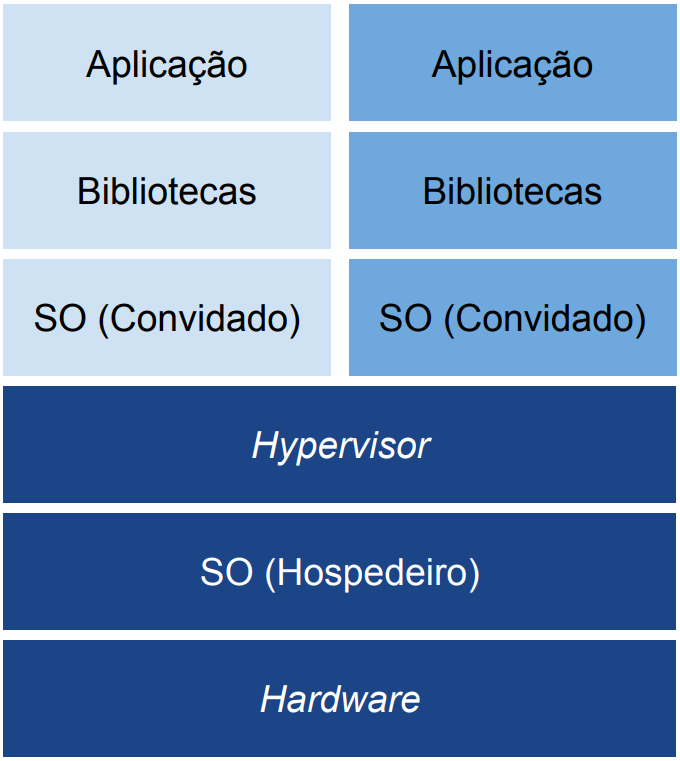
\includegraphics[width=0.8\textwidth]{virtualizacao-hypervisor.png}
        \caption{Máquinas Virtuais.}
        \label{fig:virtualizacao-hypervisor}
    \end{subfigure}
    \hspace{1mm}
    \begin{subfigure}[b]{0.45\textwidth}
        \centering
        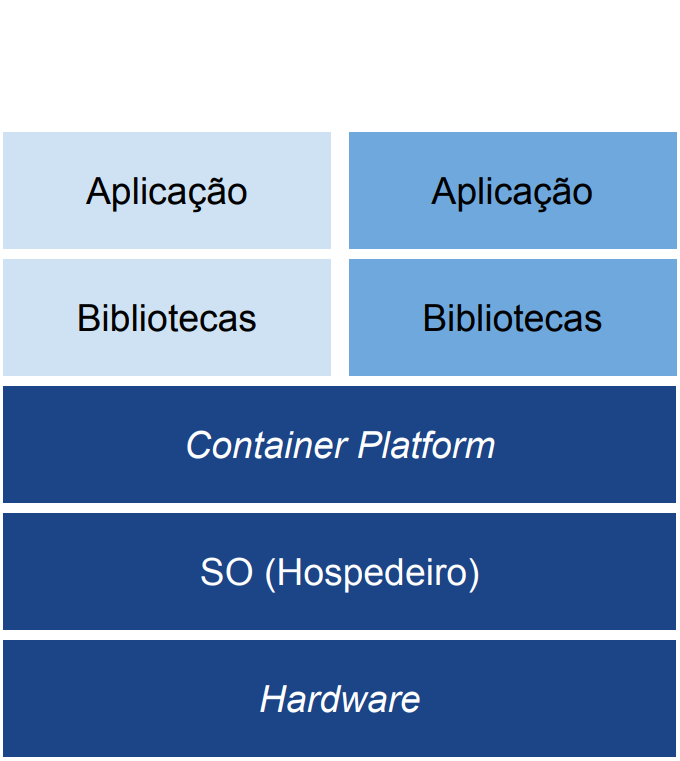
\includegraphics[width=0.8\textwidth]{virtualizacao-containers.png}
        \caption{contêineres.}
        \label{fig:virtualizacao-containers}
    \end{subfigure}
    \caption{Camadas de hardware e software em diferentes soluções de virtualização.}
    \footnotesize Fonte: Produção do próprio autor.
    \label{fig:virtualizacao-camadas-containers-e-hypervisor}
\end{figure}

\section{Computação em nuvem e borda}

Segundo os autores \citeonline{mohammed2021sufficient}, o termo ``computação em nuvem'' pode ser definida como um ambiente na Internet que permite utilizar softwares, dados e recursos de qualquer lugar. Nesse sentido, as tecnologias de virtualização foram essenciais para realização do que hoje entende-se como computação em nuvem. Assim, pode-se caracterizar três tipos básicos de modelos de serviço de computação em nuvem:
\begin{itemize}
    \item \textit{Infrastructure as a Service} (IaaS): o usuário gerencia recursos computacionais (máquinas virtuais, endereços IP, armazenamento, rede, etc).
    \item \textit{Platform as a Service} (PaaS): o usuário gerencia plataformas de computação, permitindo construir aplicações e distribuídas na rede;
    \item \textit{Software as a Service} (SaaS): o usuário tem acesso a aplicações gerenciadas por um provedor. Tais aplicações são disponibilizadas através da Internet, eliminando a necessidade do usuário de instalar softwares em seu computador pessoal.
\end{itemize}

Por outro lado, o termo ``computação em borda'' é um conceito que se refere à estratégia de trazer os serviços e aplicações de computação em nuvem para perto, geograficamente, do usuário final possibilitando um menor tempo de resposta \cite{khan2019edge}. Normalmente, os usuários finais executam as aplicações em dispositivos com capacidade limitada de processamento, o que implica no uso da nuvem para execução dos principais serviços e aplicações. Como resultado, problemas de alta latência e mobilidade são recorrentes.

Segundo os autores \citeonline{khan2019edge}, os problemas de computação em nuvem podem ser resolvidos por diferentes modelos de computação em borda. Um deles é a computação em névoa, que estende os recursos computacionais disponíveis na nuvem para a borda da rede através do uso de vários dispositivos interconectados \cite{coutinho2016nevoa}. No entanto, estender uma plataforma altamente virtualizada para borda da rede é um desafio. Isso, \recom{porqu\^{e},}{porque} envolve o uso de diferentes hardwares, protocolos de rede, grande número de dispositivos, entre outras dificuldades.

\section{Arquitetura de Microsserviços}

Uma aplicação monolítica pode ser caracterizada como um software cujos módulos não podem ser executados de forma independente \cite{dragoni2017microservices}. À medida que a complexidade da aplicação cresce, torna-se difícil realizar manutenção e localizar problemas. Além disso, uma pequena mudança em um dos seus módulos resulta na necessidade de reinicialização de toda a aplicação.

Nesse contexto, arquiteturas de microsserviços têm sido propostas como solução para os problemas encontrados em aplicações monolíticas. Segundo os autores \citeonline{dragoni2017microservices}, um microsserviço é um processo coeso e independente que interage com outros microsservicos por meio de mensagens. Nessa definição, utiliza-se o termo ``coeso'' para indicar que cada microsserviço implementa apenas funcionalidades fortemente relacionadas ao que ele realiza. Assim, uma arquitetura de microsserviços pode ser definida como uma aplicação distribuída \add{(Você não definiu o que seria uma aplicação distribuída. Talvez fosse interessante trazer a definição no primeiro parágrafo, contrapondo a definição de aplicação monolítica.)} onde todos os módulos são microsserviços. Esse tipo arquitetura de desenvolvimento tornou-se amplamente utilizada pela indústria ao possibilitar alta disponibilidade, flexibilidade, escalabilidade e velocidade. Como cada microsserviço é um processo independente, pode ser escalado conforme a necessidade, diferentemente de uma arquitetura monolítica onde seria necessário escalar todos os módulos.


\section{Kubernetes}

Kubernetes é uma plataforma \add{de} código aberto, portável e extensiva para o gerenciamento de cargas de trabalho e serviços distribuídos em contêineres \cite{google2023kubernetes}. Um \textit{cluster} Kubernetes pode ser caracterizado como um conjunto de servidores de processamento, nós, responsáveis por executar os contêineres. 

Obrigatoriamente, em um \textit{cluster}, deve existir um plano de controle a ser executado em um dos nós ou replicado em diversos. O plano de controle é responsável por gerenciar o \textit{cluster}, decidir onde alocar as aplicações, responder a eventos, etc. Os seus principais componentes são: (i) \textit{kube-apiserver}, uma API (do inglês, \textit{Application Programmable Interface}) que expõe as funcionalidades do \textit{cluster}; (ii) \textit{etcd}, um banco de dados distribuído para armazenar o estado do \textit{cluster}; (iii) \textit{kube-scheduler}, aplicação responsável por decidir em que nó cada unidade básica de escalonamento será alocada dentro do \textit{cluster}, levando com conta os recursos e restrições impostas; (iv) \textit{kube-controller-manager}, componente com os diversos controladores do \textit{cluster}.

Além disso, em todos os nós, é necessário que algumas aplicações sejam executadas para que sejam controlados pelo plano de controle. Esses componentes são: (i) \textit{kubelet}, aplicação que garante a execução dos \recom{\textit{containers}}{contêineres}; e (ii) \textit{kube-proxy}, \textit{proxy} de rede executado em cada nó que realiza o encaminhamento de trafégo de rede corretamente dentro do \textit{cluster}. Na Figura \ref{fig:kubernetes-componentes}, observa-se como esses componentes se integram e formam um \textit{cluster} para o gerenciamento de cargas de trabalho e serviços distribuídos.

\add{Em nenhum lugar está descrito \textit{kubectl} que aparece na figura. Você acha que seria interessante fazer isso?}

\begin{figure}[ht]
    \centering
    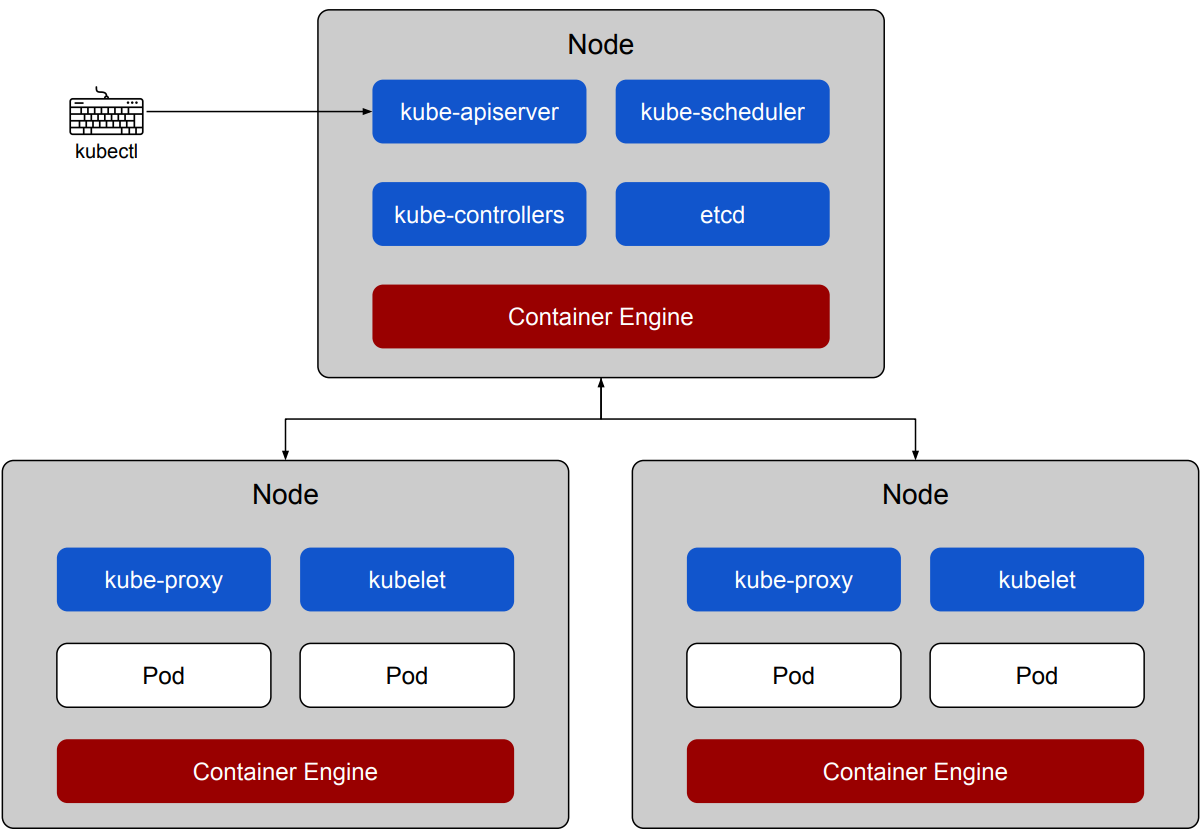
\includegraphics[width = 0.75\textwidth]{k8s-components.png}
    \caption{Componentes de um \textit{cluster} Kubernetes.}
    \footnotesize Fonte: Produção do próprio autor.
    \label{fig:kubernetes-componentes}
\end{figure}

Através da API disponibilizada pelo plano de controle, diversos recursos estão disponíveis para criação. Estes recursos podem ser entendidos como objetos ou entidades persistentes. Uma vez criado, os componentes do \textit{cluster} trabalham para garantir a sua existência. Dentre eles, tem-se:
\begin{itemize}
    \item \textit{Pod}: é o recurso mais simples, a unidade básica de um \textit{cluster} Kubernetes, e pode conter um ou mais contêineres;
    \item \textit{ReplicaSet}: recurso que garante que um número de réplicas de um determinado \textit{Pod} esteja em execução;
    \item \textit{DaemonSet}: recurso que garante um \textit{Pod} executando em cada nó do \textit{cluster};
    \item \textit{Job}: recurso que garante que um ou mais \textit{Pods} sejam executados com sucesso.
\end{itemize}

Para cada recurso, é necessário um controlador associado para garantir que o estado desejado seja alcançado. Além dos recursos disponíveis por padrão, a API do Kubernetes também permite a criação de recursos customizados. No entanto, pode ser necessário o desenvolvimento de um controlador associado para implementar a lógica de controle.

\section{Espaços Inteligentes Programáveis}

Segundo o autor \citeonline{carmo2021arquitetura}, um Espaço Inteligente é definido como um espaço físico equipado com uma rede de sensores, atuadores e serviços computacionais que atuam com o objetivo de atender as necessidades dos usuários presentes no ambiente. Além disso, o autor aponta que esses elementos devem ser gerenciados por uma infraestrutura de hardware e software responsável por coletar e analisar os dados, gerar decisões e atuar quando necessário. Para isso, uma arquitetura baseada em microsserviços com orquestração multinível centrada na observabilidade e programabilidade granular da infraestrutura é proposta, um Espaço Inteligente Programável (PIS, do inglês \textit{Programmable Intelligent Space}).

\subsection{Arquitetura}

A arquitetura proposta por \citeonline{carmo2021arquitetura} possui 4 camadas horizontais e 2 camadas transversais. Na Figura \ref{fig:pis-model-conceitual}, pode-se observar todas camadas, suas principais funções e como se relacionam.

\begin{figure}[ht]
    \centering
    \includegraphics[width= 125mm]{PIS-model.png}
    \caption{Modelo Conceitual da arquitetura do PIS.}
    \footnotesize Fonte: \citeonline{carmo2021arquitetura}
    \label{fig:pis-model-conceitual}
\end{figure}

A camada de virtualização é responsável por abstrair os recursos de hardware e torná-los disponíveis para o uso. Nesse sentido, utilizam-se softwares como \textit{Hypervisors} e plataformas de criação de contêineres nessa camada. Superior à camada de virtualização, a camada de comunicação é responsável por fornecer conectividade e interação entre as aplicações. As aplicações podem utilizar diferentes protocolos dentro do PIS, tais como HTTP (do inglês, \textit{Hypertext Transfer Protocol}) ou AMQP (do inglês, \textit{Advanced Message Queuing Protocol}). Na Seção \ref{sec:pis-comunicacao}, os detalhes de cada protocolo de comunicação são explorados.

A camada de serviços engloba as aplicações desenvolvidas, enquanto a camada de suporte à aplicação \recom{trata-se das}{corresponde às} bibliotecas e ferramentas auxiliares para o desenvolvimento delas. Já a camada de segurança tem como responsabilidade realizar controle de acesso, segurança dos dados, segurança da comunicação e gerenciamento de privacidade. Por isso, \add{essa última está} presente ao longo de todas as \recom{4}{quatro} camadas horizontais.

Por fim, tem-se a camada de gerenciamento, responsável por gerenciar os elementos de todas as \recom{4}{quatro} camadas horizontais. Para isso, deve prover as seguintes funções: (i) Orquestração e Informações multinível; (ii) Observabilidade; e (iii) Gerenciamento dos recursos. 

% \begin{itemize}

%     \item Orquestração e Informações multinível: a orquestração pode ser realizada através de \textit{softwares} como Kubernetes, que permite a alocação de contêineres em um conjunto de máquinas através de diversas estratégias. 
    
%     \item Observabilidade: pode ser definido como a capacidade de visualizar e compreender o comportamento de um sistema reunindo, processando dados do sistema e apresentando os de maneira adequada \cite{picoreti2018observability}. Aplicações podem ser implantadas em \textit{clusters} Kubernetes para permitir a coleta de métricas, \textit{logs}, rastreios. \textit{Softwares} como Prometheus, um servidor de métricas, pode ser instalado e configurado para coleta de diversas métricas do sistema (uso de CPU, memória, disco, etc). Além disso, para analisar o desempenho do sistema pode-se utilizar funções de rastreamento através da instrumentação do código e sistemas de coleta dessas informações, tais como Zipkin. Na seção \ref{sec:pis-rastreamento}, os detalhes sobre rastreamento são explorados.

%     \item Gerenciamento de recursos: através do próprio Kubernetes pode-se gerenciar os recursos que estão sendo orquestrados. Além disso, também pode-se utilizar \textit{softwares} como OpenStack para criação de máquinas virtuais.

% \end{itemize}


\subsection{Comunicação}
\label{sec:pis-comunicacao}

O protocolo HTTP é um protocolo de comunicação na camada de aplicação do modelo OSI (do inglês, \textit{Open System Interconnection}) amplamente utilizado e difundido. É baseado no padrão cliente/servidor, onde um servidor é um programa responsável por aceitar conexões de requisições de serviço e enviar respostas. Por outro lado, um cliente é uma aplicação que estabelece conexões com o servidor com o objetivo de enviar requisições \cite{berners1996hypertext}.  No contexto do protocolo HTTP, há oito tipos de requisições (também chamados de métodos HTTP) que o cliente pode iniciar. Assim, o servidor responde adequadamente a cada uma dessas requisições com um código de três dígitos informando ao cliente o \textit{status} da solicitação. A seguir, tem-se os principais métodos e as ações que realizam:

\begin{itemize}
    \item GET: usado para ler informações do servidor;
    \item PUT: usado para modificar completamente um dado no servidor ou gerar um novo dado nele;
    \item POST: usado para transferir dados ao servidor, na forma de arquivos, formulários ou outros;
    \item DELETE: usado para remover um dado especificado no servidor.
\end{itemize}

O protocolo AMQP também é um protocolo de comunicação na camada de aplicação do Modelo OSI. No entanto, é um protocolo de comunicação assíncrono orientado a mensagens baseado no padrão \textit{publish}/\textit{subscribe}. Como apontado pelos autores \citeonline{eugster2003pusub}, no padrão \textit{publish}/\textit{subscribe}, os produtores publicam mensagens em um barramento, enquanto os consumidores se subscrevem para receber mensagens com as informações que desejam. 

% NÃO SEI SE VOU DEIXAR ISSO
% Além disso, os autores \citeonline{eugster2003pusub} destacam que comunicações ponto-a-ponto e síncronas levam a aplicações rígidas e estáticas, fazendo com que a escalabilidade do sistema seja prejudicada.

A utilização do protocolo AMQP está associada à execução de uma aplicação conhecida como \textit{broker}, responsável por realizar o roteamento das mensagens dos produtores para os consumidores corretamente. Se necessário, também pode armazenar as mensagens para entregar aos consumidores quando estes estiverem disponíveis.

% O autor \citeonline{queiroz2016infraestruturaespaco} detalha o roteamento de mensagens dentro do PIS através do \citeonline{rabbitmq2023rabbitmq} como  \textit{broker}. Para implementar o padrão de comunicação \textit{publish}/\textit{subscribe}, \citeonline{rabbitmq2023rabbitmq} cria filas  para armazenar as mensagens. No entanto, apenas as filas não são suficiente. É necessário um elemento de roteamento das mensagens responsável por encaminhar corretamente cada mensagem à fila correta. Este elemento, é denominado \textit{exchange}. Além disso, a relação entre uma fila e uma \textit{exchange} é denominada \textit{binding} e podem ser entendida como uma regra de roteamento. Quando uma mensagem é enviada, esta deve possuir uma \textit{exchange} de destino. Bem como, sua identificação de roteamento, denominada \textit{routing key}.

% \begin{figure}[ht]
%     \centering
%     \includegraphics[width = 0.5\textwidth]{img/roteamento-multiplas-filas.png}
%     \caption{Representação da comunicação entre um produtor e dois consumidores, com um \textit{exchange}, duas filas e três diferentes \textit{bindings}}
%     \footnotesize Fonte: \citeonline{queiroz2016infraestruturaespaco}.
%     \label{fig:roteamento-multiplas-filas}
% \end{figure}

% Considere a Figura \ref{fig:roteamento-multiplas-filas}, que o autor \citeonline{queiroz2016infraestruturaespaco} aponta como exemplo. O produtor, P1, envia as mensagens à \textit{exchange} X1. Os consumidores C1 e C2 possuem as suas filas associadas, respectivamente, Q1 e Q2 . Observe que, a fila Q1 possui um \textit{binding}, B1, com a \textit{exchange} X1. Enquanto, a fila Q2 possui dois \textit{bindings}, B1 e B2, com a \textit{exchange} X1. Assim, se uma mensagem for enviada ao \textit{broker} com a \textit{exchange} X1 de destino e \textit{routing key} B1, ambas as filas Q1 e Q2 irão receber a mensagem. No entanto, se uma mensagem for enviada ao \textit{broker} com a \textit{exchange} X1 de destino e \textit{routing key} B2, apenas a fila Q2 irá receber a mensagem.

% Existem diversas categorias de \textit{exchanges}, a mencionada no exemplo anterior é do tipo \textit{direct}. Onde, a mensagem é encaminhada para a fila de acordo com o \textit{binding}. No entanto, este tipo de \textit{exchange} possui limitações. Para realizar um roteamento de mensagens baseados em múltiplos critérios, uma \textit{exchange} do tipo \textit{topic} deve ser utilizada. Nesse tipo de \textit{exchange}, mensagens enviadas ao \textit{broker} não podem ter uma \textit{routing key} arbitrária - deve ser uma lista de palavras separadas por pontos.

% Assim, na camada de comunicação do PIS são utilizadas \textit{exchanges} do tipo \textit{topic} para permitir uma maior flexibilidade de roteamento das mensagens ao construir um lista de palavras com tipos e subtipos, tais como \textit{CameraGateway.0.Frame}. A primeira palavra representa o serviço, a segunda o identificador da câmera e a terceira o tipo de informação da câmera, no caso uma imagem. Para receber imagens de todas as câmeras que enviam mensagem a \textit{exchange}, basta se subscrever com a seguinte regra: \textit{CameraGateway.*.Frame}.

\subsection{Observabilidade}
\label{sec:observabilidade}

O termo ``observabilidade'' pode ser definido como a capacidade de visualizar e compreender o comportamento de um sistema através da coleta e processamento de dados \cite{picoreti2018observability}. São utilizados três tipos de dados principais para prover informações de observabilidade de um sistema: \textit{logs}, métricas e \textit{traces}.

Os \textit{logs} são linhas de texto estruturadas e não estruturadas que um sistema gera quando uma parte específica do código é executada. Em outras palavras, um \textit{log} é um registro de um evento em um aplicação. Geralmente, são coletados por uma camada de agregação para ser pré-processado e, em seguida, persistido para posterior processamento e análise. Por isso, os \textit{logs} são comumente utilizados para descobrir problemas e analisar comportamentos imprevisíveis do sistema.

Por outro lado, as métricas podem ser definidas como números coletados periodicamente formando uma série temporal. Dessa forma, ajudam a mostrar tendências sobre o comportamento e performance do sistema ao longo do tempo. Para isso, também são coletadas por uma camada de agregação periodicamente para processamento e persistência.

Já os \textit{traces} podem ser entendidos como uma forma de observabilidade do sistema que permite determinar a causalidade entre eventos de diversos aplicações, bem como extrair medidas de desempenho. Para isso, cada serviço deve contribuir propagando um contexto, que deve ser enviado diretamente a uma ferramenta responsável por correlacionar cadeia de eventos e apresentar aos usuários. Na Figura \ref{fig:exemplo-trace}, tem-se um exemplo de \textit{trace} e sua respectiva árvore de \textit{spans} (unidade básica de trabalho, um registo temporal com início e fim associado a alguma função ou serviço) indicando a causalidade entre eles.

\begin{figure}[ht]
    \centering
    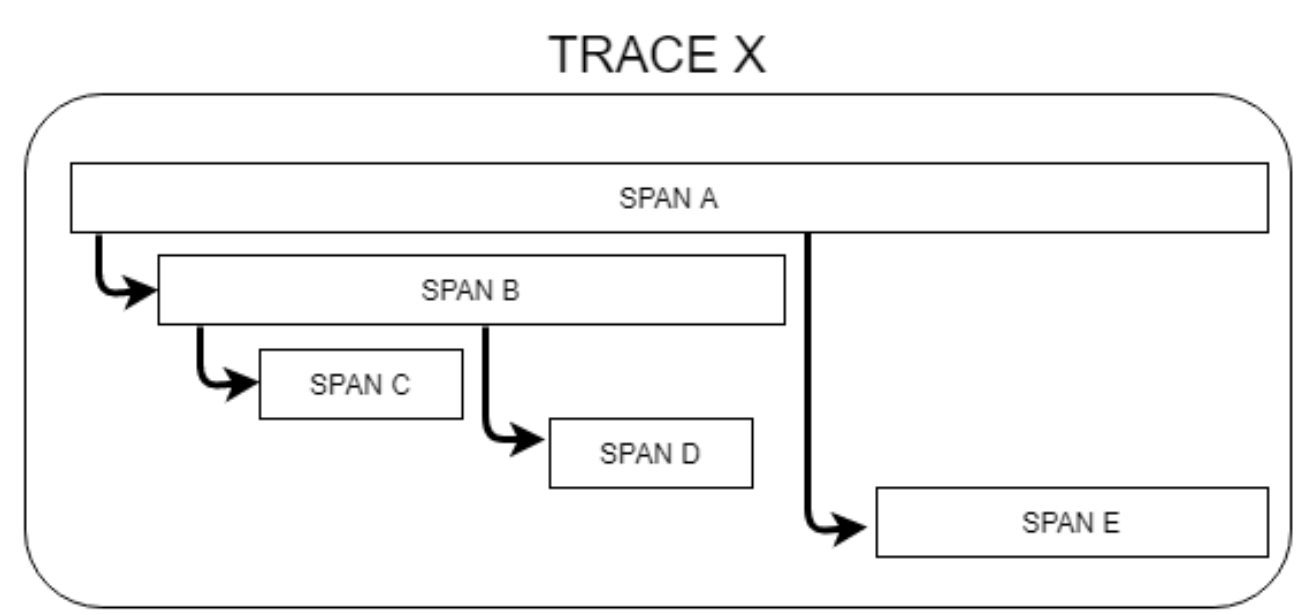
\includegraphics[width=0.5\textwidth]{images/exemplo-trace.png}
    \caption{Exemplo de rastreamento.}
    \footnotesize Fonte: \citeonline{cotta2020medicao}.
    \label{fig:exemplo-trace}
\end{figure}

Por ser um método baseado em anotações, nesse tipo de solução há necessidade de instrumentação do código. Ou seja, é necessário informar no código onde a medição começa e termina \cite{sigelman2010tracing}.

% Assim, em um sistema de rastreamento tem-se \cite{cotta2020medicao} \cite{sigelman2010tracing}:

% \begin{itemize}
%     \item \textit{Annotations}: unidade básica de informação. Pode ser do tipo \textit{timing}, com medições de tempo, ou do tipo \textit{tags} com informações gerais na forma de chaves e valores.
%     \item \textit{Spans}: unidade básica de trabalho, um registo temporal com início e fim associado a alguma função ou serviço. Ou seja, um conjunto de \textit{annotations} do tipo \textit{tags} (para identificar a medição) e \textit{timing} (para medir o tempo decorrido).
%     \item \textit{Trace}: é uma coleção de \textit{spans} na forma de uma árvore, onde os nós representam os \textit{spans} e as arestas representam a relação de causalidade.
% \end{itemize}

% Uma vez realizada a instrumentação do código, os tempos de processamento podem ser observados consultando na interface do Zipkin. Através do trabalho desenvolvido pelo o autor \citeonline{cotta2020medicao}, pode-se obter os tempos de comunicação entre as aplicações através de modificações na camada que implementa a comunicação no PIS. No entanto, para que isso seja possível é necessário configurar corretamente uma ferramenta de sincronização de relógios. Por isso, todos os servidores e dispositivos robóticos serão configurados através da ferramente Chrony, que implementa a sincronização de relógios de diferentes dispositivos através do protocolo NTP.


% \subsection{Processo de orquestração}

% \begin{figure}[ht]
%     \centering
%     \includegraphics[width= 125mm]{img/PIS_orquestracao.png}
%     \caption{Processo de orquestração do PIS.}
%     \footnotesize Fonte: \citeonline{carmo2021arquitetura}
%     \label{fig:pis-orquestracao}
% \end{figure}


\section{Trabalhos relacionados}

 No trabalho proposto pelos autores \citeonline{santoro2017foggy}, uma plataforma de orquestração de aplicações para computação em borda é proposta. De acordo com os requisitos impostos durante o momento de instalação das aplicações, estas eram direcionadas de forma à atender os requisitos geográficos ou de capacidade da rede. Assim, era possível orquestrar aplicações tanto em nuvem quanto em borda (o mais próximo do cliente). Além disso, uma aplicação de detecção facial é apresentada no contexto de cidades inteligentes e alguns cenários são explorados. Ao orquestrar a aplicação de detecção facial perto do cliente, há uma diminuição da largura de banda utilizada na conexão com a nuvem e um menor tempo de resposta. No entanto, os autores não apontam o uso de ferramentas de observabilidade, que poderiam ser utilizadas para atualizar a instalação dessas aplicações na plataforma dinamicamente. Também não é abordado no artigo aspectos relevantes de como a comunicação ocorre, por exemplo, se é um modelo de comunicação baseado em mensagens.

Já no trabalho proposto pelos autores \citeonline{mohamed2017uavfog}, uma plataforma de computação em borda baseada no uso de VANTs para aplicações IoT é proposta. Um VANT equipado com os recursos de computação pode viajar para um local específico quando necessário e permanecer nesse local para oferecer suporte aos aplicativos IoT locais. Cada VANT possui um \textit{broker} com um conjunto de aplicações disponíveis. Assim, caso o serviço desejado pela aplicação IoT local não esteja disponível a bordo, a aplicação pode solicitar à um \textit{broker} em nuvem através do próprio dispositivo. Nesse contexto, os autores mostram que ao colocar aplicações no VANT responde-se de forma mais rápida às requisições ao eliminar a necessidade de consulta em nuvem. No entanto, os autores também não exploram ferramentas \recom{uso}{de} observabilidade e como essas poderiam ser utilizadas dentro da plataforma proposta para uma orquestração inteligente dessas aplicações (em nuvem ou a bordo do VANT).

Um outro trabalho que propõe o uso de VANTs no contexto de computação em borda, foi proposto pelos autores \citeonline{sanchez2021uav}. O objetivo é gerenciar as operações de VANTs remotamente e prover conectividade aos dispositivos locais. Para isso, esses dispositivos robóticos são capazes de prover uma rede 4G e assim disponibilizar conectividade aos dispositivos IoT locais. Também foi proposta a integração nos VANTs de uma plataforma de virtualização de contêineres para a implantação dos serviços necessários. Assim, algumas aplicações são orquestradas a bordo e outras em nuvem. No entanto, os autores não exploram o uso de ferramentas de observabilidade e possibilidade de realizar algum processamento a bordo para execução de tarefas (por exemplo, seguimento de padrões). A plataforma no dispositivo robótico funciona como uma ponte para nuvem, que é responsável por controlá-lo.

O conceito de observabilidade multinível \add{em Espaços Inteligentes} foi introduzido pelo trabalho proposto pelos autores \citeonline{picoreti2018observability}, considerando métricas tanto da infraestrutura quanto das aplicações para melhorar o escalonamento e orquestração automática de aplicações em ambientes de nuvem. Os autores obtiveram melhores resultados com o uso de métricas como tempo de resposta, medido pela aplicação, do que com a utilização de métricas como taxa de utilização de CPU. Além do uso de métricas para o escalonamento, foi apontado como trabalhos futuros \recom{pelos}{por} \citeonline{picoreti2018observability} o uso de \textit{traces} para a identificação de gargalos no sistema e escalonamento das aplicações como forma de mitigação de problemas relacionados à alta latência. Assim, os autores \citeonline{tzanettis2022fusion} proposeram um \textit{framework} de orquestração baseado nos 3 pilares da observabilidade: métricas, \textit{traces} e \textit{logs}. Ao levar em conta tanto as métricas quanto os \textit{traces}, o \textit{framework} de observabilidade é capaz de responder a problemas de latência e escalonar os serviços adequadamente. 

Nesse sentido, o presente trabalho visa estender a plataforma de orquestração de contêineres para os dispositivos robóticos permitindo a computação em borda de aplicações, tal como realizado pelos trabalhos propostos pelos autores \citeonline{santoro2017foggy},  \citeonline{mohamed2017uavfog} e \citeonline{sanchez2021uav}, \recom{e tambem}{assim como} a expansão da abrangência do Espaço Inteligente através dos sensores embarcados. No entanto, \recom{se difere ao }{sua principal diferença está no fato de} utilizar as informações multinível, disponibilizadas pelos serviços que fazem parte do PIS, para gerenciar onde devem ser orquestrados, em nuvem ou em borda, a fim de atender os requisitos das aplicações com utilização racional dos recursos de infraestrutura. Diferentemente dos trabalhos propostos por \citeonline{picoreti2018observability} e \citeonline{tzanettis2022fusion}, nesse trabalho não se pretende utilizar as informações multinível para escalonamento, mas para a correta alocação em nuvem ou em borda. Para validação, pretende-se utilizar uma aplicação de detecção de marcadores visuais e controlar a sua orquestração de acordo com o tempo de resposta.


% atender os requisitos da aplicação com utilização racional dos recursos computacionais
% colocar cenário de expansão da abragencia do PIS também neste paragráfio, deixar a parte do cenário bem claro

% ultima frase: para validação...

% Nesse sentido, o presente trabalho visa estender a plataforma de orquestração de contêineres para os dispositivos robóticos permitindo à computação em borda de aplicações, tal como realizado pelos trabalhos relacionados apresentados anteriormente. No entanto, se difere ao utilizar as informações multinível disponibilizadas pelos serviços que fazem parte do PIS para gerenciar onde devem ser orquestrados, em nuvem ou em borda, a fim de garantir alta disponibilidade para os sistemas com utilização racional dos recursos de infraestrutura. Observe que, no caso aqui apresentado neste trabalho, não basta utilizar métricas de infraestrutura como uso de CPU e memória. Faz-se necessário orquestrar de acordo com métricas características da aplicação, como o tempo de resposta total.



%%%%%%%%%%%%%%%%%%%%%%%%%%%%%%%%%%%%%%%%%%%%%%%%%%%%%
%%%%%%%%%%%%%%%%%%%%%%%%%%%%%%%%%%%%%%%%%%%%%%%%%%%%%
%%%%%%%%%%%%%%%%%%%%%%%%%%%%%%%%%%%%%%%%%%%%%%%%%%%%%

\ifisTipoDocumento
\chapter[Metodologia e etapas de desenvolvimento]{Metodologia e etapas de desenvolvimento}
% escrever um textinho falando o que vem a seguir nas próximas subseções
\section{Metodologia Adotada}

Neste trabalho, pretende-se modificar e desenvolver novas aplicações. Além disso, integrá-las e validá-las através de experimentos no PIS localizado na UFES no Laboratório de Visão Computacional e Robótica.

Para integrar dispositivos robóticos dentro do PIS, faz-se necessário adicionar o sistema embarcado que os controlam dentro da plataforma de orquestração de contêineres como nós de computação em borda. Assim, obtendo um \textit{cluster} formado por nós de computação em nuvem (\textit{Datacenter} presente no laboratório) e nós de computação em borda.

Para isso, pretende-se utilizar uma Raspberry 4B, como exemplo de dispositivo para computação em borda. Ao integrá-la \add{ao} \textit{cluster} Kubernetes já existente no laboratório, pretende-se variar a largura de banda da conexão disponível com a nuvem. Dessa forma, ao orquestrar as aplicações no \textit{cluster}, pretende-se analisar as informações multiníveis disponibilizadas pelas ferramentas de observabilidade presentes no PIS e desenvolver um controlador responsável por avaliar onde as aplicações devem ser executadas, em nuvem ou em borda, a fim de atender os requisitos das aplicações com utilização racional dos recursos de infraestrutura.

É importante notar que, para \recom{ser possivel}{se} obter as informações desejadas, é necessário que as aplicações sejam instrumentadas corretamente. Ou seja, é necessário modificar as aplicações inserindo blocos de códigos responsáveis por enviar as informações desejadas, tais como tempo de resposta.

\begin{figure}[ht]
    \centering
    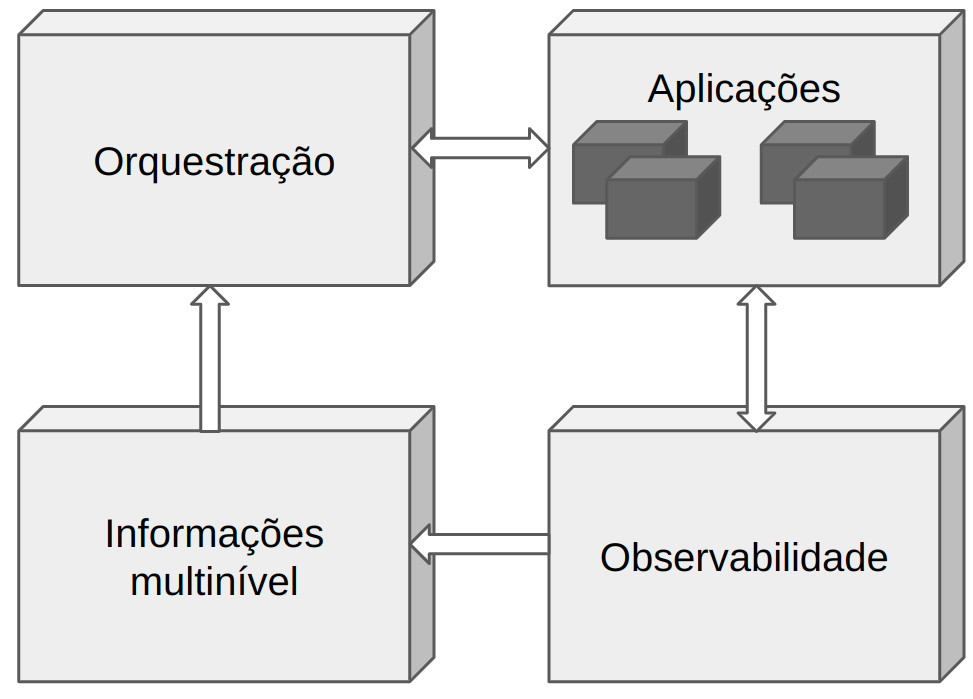
\includegraphics[width=80mm]{images/metodologia.png}
    \caption{Metodologia adotada.}
    \label{fig:metodologia}
\end{figure}


Na Figura \ref{fig:metodologia}, pode-se observar como \recom{pretende-se}{se pretende} realizar este trabalho. Tanto as aplicações quanto as ferramentas de observabilidade se comunicam a fim de mensurar as informações desejadas. Por sua vez, as ferramentas de observabilidade disponibilizam essas informações para o PIS, tanto informações características das aplicações, como o tempo de resposta, quanto informações da infraestrutura, como o uso de CPU e memória. A partir dessas informações, pretende-se desenvolver um controlador integrado à plataforma de orquestração de contêineres para alocar corretamente as aplicações.

\section{Cronograma de Trabalho}

O trabalho será desenvolvido conforme as etapas apresentadas a seguir.

\begin{itemize}
\item 
\textbf{Atividade 1. Revisão bibliográfica}:
(\textit{i}) estudo sobre computação em borda e espaços inteligentes;
(\textit{ii}) revisão a respeito das técnicas para computação em borda no contexto de Espaços Inteligentes.

\item 
\textbf{Atividade 2. Criar e configurar uma plataforma para computação em borda e em nuvem}:
(\textit{i}) criar uma plataforma de orquestração de contêineres com dispositivos robóticos como nós de computação em borda e servidores como nós de processamento em nuvem;
(\textit{ii}) configurar a plataforma.

\item 
\textbf{Atividade 3. Instalar as aplicações de suporte ao PIS}:
(\textit{i}) realizar a instalação dos softwares que compõe o PIS e configurar a integração entre nuvem e borda.

\item 
\textbf{Atividade 4. Adaptação das aplicações do sistema}:
(\textit{i}) adaptação das aplicações que irão compôr o sistema para expôr o tempo de resposta total;
(\textit{ii}) construção das imagens de contêineres para execução em borda e em nuvem;

\item 
\textbf{Atividade 5. Desenvolvimento de um controlador para realizar o gerenciamento das aplicações}:
(\textit{i}) determinação do tempo de resposta total em borda e em nuvem;
(\textit{ii}) desenvolver um controlador responsável por decidir onde orquestrar as aplicações (em nuvem ou em borda) com base no tempo de resposta;
(\textit{ii}) escrever a documentação do controlador;

\item 
\textbf{Atividade 6. Validação do controlador desenvolvido}:
(\textit{i}) realizar experimentos variando a largura de banda disponível em borda e verificar como o controlador orquestra as aplicações;
(\textit{ii}) gerar gráficos e apresentar resultados do sistema em funcionamento.

\item 
\textbf{Atividade 7. Redação do projeto de graduação}:
(\textit{i}) expandir o referencial teórico;
(\textit{ii}) descrever a arquitetura do sistema;
(\textit{iii}) apresentar e discutir os resultados.

\item 
\textbf{Atividade 8. Revisão do projeto de graduação}:
(\textit{i}) revisar o texto junto à orientadora e coorientador;
(\textit{ii}) corrigir os possíveis erros.

\item 
\textbf{Atividade 9. Defesa do projeto de graduação}:
(\textit{i}) após a aprovação da escrita, a defesa do projeto de graduação será realizada.

\end{itemize}

%1. DEFINIMOS O NUMERO DE MESES NOS QUAIS SERÁ IMPLEMENTADO O PROJETO
\newcommand{\DuracionPlanoMeses}{6}

% 2. DEFINIMOS AS ATIVIDADES COMO COMANDOS VIA \newcommand{\name_comand}{value}
% primeira atividade
\newcommand{\AtvAlgRotI}{Revisão bibliográfica}
% segunda atividade
\newcommand{\AtvAlgRotII}{Criar e configurar uma plataforma para computação em borda e em nuvem}
% terceira atividade
\newcommand{\AtvAlgRotIII}{Instalar as aplicações de suporte ao PIS}
% quarta atividade
\newcommand{\AtvAlgRotIV}{Adaptação das aplicações do sistema}
% quinta atividade
\newcommand{\AtvAlgRotV}{Desenvolvimento de um controlador para realizar o gerenciamento das aplicações}
% sexta atividade
\newcommand{\AtvAlgRotVI}{Validação do controlador desenvolvido}
% setima atividade
\newcommand{\AtvAlgRotVII}{Redação do projeto de graduação}
% oitava atividade
\newcommand{\AtvAlgRotVIII}{Revisão do projeto de graduação}
% nona atividade
\newcommand{\AtvAlgRotIX}{Defesa do projeto de graduação}


% 3. DEFINIMOS OS ROTULOS DAS AS ATIVIDADES A SER USADAS NO DIAGRAMA DE GANTT USANDO O COMANDO \newcommand{\name_comand}{value}
%ROTULOS DE ATIVIDADES
\newcommand{\RTLAtvAlgRotI}{ATV 1} %rotulo da primeira atividade
\newcommand{\RTLAtvAlgRotII}{ATV 2} %rotulo da segunda atividade
\newcommand{\RTLAtvAlgRotIII}{ATV 3} %rotulo da terceira atividade
\newcommand{\RTLAtvAlgRotIV}{ATV 4} %rotulo da quarta atividade
\newcommand{\RTLAtvAlgRotV}{ATV 5} %rotulo da quinta atividade
\newcommand{\RTLAtvAlgRotVI}{ATV 6} %rotulo da sexta atividade
\newcommand{\RTLAtvAlgRotVII}{ATV 7} %rotulo da sétima atividade
\newcommand{\RTLAtvAlgRotVIII}{ATV 8} %rotulo da oitava atividade
\newcommand{\RTLAtvAlgRotIX}{ATV 9} %rotulo da nona atividade


%4. COMENTARIOS SOBRE O DIAGRAMA DE ATIVIDADES
Apresenta-se nesta seção uma previsão do cronograma do plano de trabalho. Esse projeto será realizado no período correspondente ao semestre 2023/2, aproximadamente \DuracionPlanoMeses\ meses. A data de início do projeto será 21 de julho de 2023 e a data prevista para encerramento, 16 de dezembro de 2023. Na Tabela \ref{Tab1}, são detalhadas as atividades que se pretende realizar para o desenvolvimento do plano de trabalho. Assim, na primeira coluna da tabela são definidos os rótulos de cada atividade e na segunda coluna é feita uma descrição da atividade que se pretende realizar. Finalmente, na Figura \ref{fig:gaant-cronograma} é apresentado o diagrama de tempo das atividades indicadas na Tabela \ref{Tab1}.


%5. CRIAÇÃO DA TABELA DE ATIVIDADES, OBSERVE QUE AQUI SÃO USADOS OS COMANDOS DAS ATIVIDADES
\begin{table}[!htbp]
\begin{center}\begin{tabular}{c|p{13.50cm}}
\hline
Rótulo  & Atividade \\ 
\hline
\hline
\RTLAtvAlgRotI & \AtvAlgRotI \\ 
\hline 
\RTLAtvAlgRotII & \AtvAlgRotII \\ 
\hline 
\RTLAtvAlgRotIII & \AtvAlgRotIII \\ 
\hline
\RTLAtvAlgRotIV & \AtvAlgRotIV \\ 
\hline
\RTLAtvAlgRotV & \AtvAlgRotV \\
\hline
\RTLAtvAlgRotVI & \AtvAlgRotVI \\
\hline
\RTLAtvAlgRotVII & \AtvAlgRotVII \\
\hline 
\RTLAtvAlgRotVIII & \AtvAlgRotVIII \\
\hline 
\RTLAtvAlgRotIX & \AtvAlgRotIX \\
\hline 
\end{tabular}
\end{center}
\caption{
\footnotesize
Lista de atividades. 
}
\label{Tab1}
\end{table}

%6. CRIAÇÃO DO DIAGRAMA DE GANTT DAS ATIVIDADES, OBSERVE QUE AQUI SÃO USADOS OS COMANDOS DOS  ROTULOS DAS ATIVIDADES
\begin{figure}[!htbp]
\begin{center}
\begin{ganttchart}[
x unit = 0.55cm,
y unit title=0.5cm,
y unit chart=0.5cm,
hgrid,vgrid,
title label anchor/.style={below=-1.6ex},
title height=1,
bar/.style={fill=gray!50},
%group/.style={draw=black},
incomplete/.style={fill=white},
progress label text={},
bar height=0.7,
%group right shift=0,
group top shift=.6,
group height=.3,
group peaks width=.2]{1}{24}
%labels
\gantttitle{2023}{24}\\
\gantttitle{\tiny JUL}{4}
\gantttitle{\tiny AGO}{4} 
\gantttitle{\tiny SET}{4} 
\gantttitle{\tiny OUT}{4} 
\gantttitle{\tiny NOV}{4} 
\gantttitle{\tiny DEZ}{4}\\
%tasks

% Tercceira técnica
\ganttbar[bar/.style={fill=black},bar label font=\color{black}]{\RTLAtvAlgRotI}{1}{8} \\
\ganttbar[bar/.style={fill=black},bar label font=\color{black}]{\RTLAtvAlgRotII}{3}{4} \\
\ganttbar[bar/.style={fill=black},bar label font=\color{black}]{\RTLAtvAlgRotIII}{5}{6} \\
\ganttbar[bar/.style={fill=black},bar label font=\color{black}]{\RTLAtvAlgRotIV}{7}{8} \\
\ganttbar[bar/.style={fill=black},bar label font=\color{black}]{\RTLAtvAlgRotV}{9}{12} \\
\ganttbar[bar/.style={fill=black},bar label font=\color{black}]{\RTLAtvAlgRotVI}{13}{16} \\
\ganttbar[bar/.style={fill=black},bar label font=\color{black}]{\RTLAtvAlgRotVII}{5}{20} \\
\ganttbar[bar/.style={fill=black},bar label font=\color{black}]{\RTLAtvAlgRotVIII}{17}{20} \\
\ganttbar[bar/.style={fill=black},bar label font=\color{black}]{\RTLAtvAlgRotIX}{21}{22} \\

\end{ganttchart}
\end{center}
\caption{Diagrama de tempo das atividades a \recom{efetuar}{serem realizadas} para o desenvolvimento do plano de trabalho. }
\label{fig:gaant-cronograma}
\end{figure}
\else
\chapter[Proposta]{Proposta}
% Ajustar esse \vspace de acordo com o necessário

\textbf{1. \txr{COMENTARIO GERAL}}. Muitos trabalhos em ML estão centrados em um novo modelo, abordagem ou algoritmo, e efetuar uma descrição clara é fundamental. Assim, você deve pensar cuidadosamente em comunicar as características essenciais de sua proposta.

\section{Introdução}

\textbf{1. \txr{Objetivo do capitulo}}
Neste capítulo é apresentado o problema específico a solucionar, o sistema proposto para a solução do problema em estudo.
\textbf{2. \txr{Temas a tratar}}
Sendo assim, o capítulo divide-se em três seções além desta introdução. 
Na primeira seção, é descrito o sistema proposto baseado no uso de xxxx, além de uma descrição do xxxxx.

\fi

%%%%%%%%%%%%%%%%%%%%%%%%%%%%%%%%%%%%%%%%%%%%%%%%%%%%%
%%%%%%%%%%%%%%%%%%%%%%%%%%%%%%%%%%%%%%%%%%%%%%%%%%%%%
%%%%%%%%%%%%%%%%%%%%%%%%%%%%%%%%%%%%%%%%%%%%%%%%%%%%%

\ifisTipoDocumento
\chapter[Alocação de Recursos]{Alocação de Recursos}
\section{Recursos Materiais}

\textbf{Material bibliográfico.} O material bibliográfico utilizado é composto principalmente por periódicos científicos, artigos e livros. Este material estará disponível para o autor \recom{do}{desse} trabalho das seguintes maneiras: fisicamente, via Biblioteca Central da UFES, e eletronicamente, via rede de Internet da UFES, permitindo o acesso ao acervo eletrônico próprio da universidade e ao acervo cujo acesso tenha sido adquirido pela universidade.

\section{Recursos Computacionais}

\textbf{Recursos de Software}
%\textbf{1. \txr{Descrição das ferramentas de programação usadas}}

Na etapa de criação e configuração da plataforma de orquestração de contêineres pretende-se utilizar o software Kubernetes, \recom{. Alem disso,}{além de} todo o conjunto de softwares, tais como RabbitMQ e Zipkin, que compõem a plataforma do PIS. Já durante as etapas de adaptação das aplicações do sistema, desenvolvimento e validação do controlador proposto será utilizada a linguagem de programação em Python e o conjunto de ferramentas de suporte à aplicação do PIS previamente desenvolvido. Além disso, todas aplicações devem ser empacotadas na forma de contêineres utilizando o software Docker.


\textbf{Recursos de Hardware}
%\textbf{2. \txr{Descrição do hardware usado}}

Como dispositivo IoT, pretende-se utilizar uma Raspberry model B com as seguintes configurações: (i) sistema operacional Linux, distribuição Ubuntu Server 22.04; (ii) \recom{processor}{processador} Cortex-A72 (ARM v8) 64-bit SoC, 1.5GHz com 4 núcleos físicos; (iii) memória SDRAM de 4GB LPDDR4 3200MHz; (iv) conexão Wi-Fi de 2.4 GHz e 5.0 GHz IEEE 802.11ac; (v) cartão de memória de 32GB (classe 10, até 80 MB/s); (v) Raspberry Pi Camera Module 2. 

Além disso, pretende-se utilizar um \textit{datacenter} presente no laboratório para realização dos testes de validação do sistema proposto. Neste \textit{datacenter}, a máquina com as seguintes configurações será utilizada como máquina de computação de nuvem: (i) sistema operacional Linux, distribuição Ubuntu Server 22.04; (ii) \recom{processor}{processador} Intel Xeon, 3.2GHz com 28 núcleos físicos; (iii) memória DDR4 de 64GB; (iv) conexão ethernet de 1GHz; (v) SSD de 480GB; (iv) 3 NVIDIA GeForce RTX 3060 e 1 NVIDIA GeForce RTX 3090.

\else
\chapter[Resultados]{Resultados}
{\txr{COMENTARIO GERAL}} Neste capítulo deverão ser descritos os recursos usados para a realização do projeto (equipamentos, material bibliográfico, programas de simulação, etc.), bem como aspectos relativos à disponibilidade ou não dos mesmos para a realização do estudo. Caso a disponibilidade de algum recurso seja limitada, ou esteja vinculada a alguma data de entrega, fator externo ou, até mesmo, a outro projeto, tal informação deve ser apresentada de forma explícita e clara nesta seção. O atraso ou a indisponibilidade deste recurso afetará diretamente o cronograma de execução do projeto, fato que deve ser cuidadosamente avaliado na construção do cronograma.

\section{Introdução}

\textbf{1. \txr{Objetivo do capitulo}}
Neste capítulo serão apresentados os resultados obtidos.....
\textbf{2. \txr{Temas a tratar}}
De tal modo, o capitulo inicia descrevendo o banco de dados utilizado para treinamento e teste das abordagens propostas, 
também são apresentados todos os resultados obtidos em diferentes etapas do processo, mostrando a evolução obtida a partir da implementação de algumas técnicas apresentadas anteriormente. 
E por fim, é feita uma análise destes resultados e uma comparação com os resultados obtidos por outros trabalhos semelhantes com o intuito de validar as abordagens propostas.


%\textbf{3. \txr{Descrição de algumas peculiaridades da implementação}}
% Como a capacidade da memória RAM não era suficiente para suportar a banco de dados por completo, durante a etapa de treinamento a taxa de \textit{Swap} entre a memória e o disco rígido aumentava drasticamente. 
% Com isso, uma vez que a unidade de armazenamento não era de estado sólido, o tempo de carga do próximo \textit{batch} a ser treinado era considerado grande se comparado com a rapidez a qual a GPU o processava.  Provocando uma ociosidade da mesma devido a essa espera. 
% Sendo assim, foi realizado um processo de pré-carga dos dados utilizando as bibliotecas próprias do \textit{Tensorflow}. Para isso, todas as imagens do conjunto de treino foram serializadas em um único arquivo com extensão \textit{tfrecords}, utilizando o protocolo de serialização \textit{Protobuf}\footnote{ https://github.com/google/protobuf}. Dessa forma, 7 \textit{threads} ficaram responsáveis por carregar imagens em um \textit{buffer} de tamanho pré-definido, enquanto que, paralelamente, a rede estava sendo treinada na GPU. Com o uso desse procedimento, a média de tempo de ociosidade da GPU caiu de cerca de $40\%$ para menos de $10\%$, o que possibilitou acelerar ainda mais o treinamento. 

% \textbf{4. \txr{Descrição dos valores dos hiperparâmetros da rede}}
% A seguir, são apresentados os valores dos hiperparâmetros usados para a rede CNN e o algoritmo \textit{graph cut}.
% \noindent \textit{Em relação à CNN:} a taxa de aprendizado usada tem valor $0.01$, com decaimento exponencial de $0.95$. 
% A camada totalmente conectada tem seus pesos regularizados usando norma L2.
% A busca por esses parâmetros foi empírica.
% \noindent \textit{Em relação ao algoritmo \textit{graphcut}:} considerando que são dois parâmetros $\lambda$ e $\sigma$ a serem estimados, a busca do valor desses parâmetros foi feita usando busca exaustiva. Os valores de $\sigma$ e $\lambda$ usados são: $\sigma \in \left \{ 1,15,30,45,50 \right \}$ e $\lambda \in \left \{ 1,25,50,75,100 \right \}$. 
% Para cada valor de $\sigma$ e $\lambda$ usados, foram calculadas as métricas.

\section{Recursos Computacionais}

\textbf{Recursos de \textit{Software}}
\input{Software}

\textbf{Recursos de \textit{Hardware}}
\input{Hardware}

\textbf{Base de dados xxxx.}
\input{DataBase}

\section{Experimentos}
\subsection{Métricas}

\textbf{1. \txr{Aqui as métricas usadas para a avaliação da proposta devem ser descritas}}
Considerando que a segmentação a nível de pixels foi modelado como um problema de classificação binária, a avaliação aqui utilizada será feita via as seguintes métricas: 
(\textit{i}) acurácia ($Ac$), que avalia a capacidade da técnica de classificar corretamente os pixels como objeto ou fundo; 
(\textit{ii}) sensibilidade ($Se$), que avalia a capacidade da técnica em classificar corretamente os pixels como objeto; 
(\textit{iii}) Precisão ($Pr$), que avalia a capacidade da técnica em classificar corretamente as; 
e finalmente a medida $F$ que é a média harmônica entre a sensibilidade e especificidade. As relações que definem essas métricas são apresentadas nas Equações \eqref{eq:ac} – \eqref{eq:f1}, onde: 
$VP$ são os verdadeiros positivos (número de pixels corretamente classificados pela técnica como objeto), 
$VN$ são os verdadeiros negativos (número de pixels corretamente classificados pela técnica como fundo), 
$FP$ são os falsos positivos (número de pixels classificados erroneamente pela técnica como objeto), e 
$FN$ são falsos negativos (número de pixels classificados erroneamente pela técnica como fundo). 
\begin{eqnarray}
\label{eq:ac}
Ac &=& \frac{VP + VN}{VP + VN + FP + FN}\\
\label{eq:se}
Se &=& \frac{VP}{VP + FN}\\
\label{eq:es}
Pr &=& \frac{VP}{VP + FP}\\
\label{eq:f1}
F_1 &=& 2\frac{Se.Pr}{Se + Pr}.
\end{eqnarray}

\subsubsection{Avaliação na XXXX}

\textbf{1. \txr{Aqui devem ser descritos os experimentos implementados e os resultados obtidos em função das métricas de desempenho definidas na seção anterior}}
Na Tabela \ref{resultados_simplificados} é possível visualizar os resultados obtidos na classificação dos ROIs extraídos manualmente em normais ou cancerígenos. A abordagem atinge uma acurácia de $99,41\%$. 
Também é possível observar uma grande evolução nos resultados ao se acrescentar o \textit{highboost} na etapa de pré-processamento das imagens que possui a capacidade de destacar as bordas que são características relevantes para esta aplicação. 
Além disso, a aplicação do \textit{data augmentation} conseguiu melhorar ainda mais os resultados, chegando-se a resultados finais bons se comparados à outros trabalhos semelhantes, como é possível observar na tabela \ref{comparacao_resultados_simplificada}.

\begin{table}[h]
\centering
\caption{Resultados para a abordagem semi-automática, na classificação dos ROIs em normais ou cancerígenos.}
\begin{tabular}{l|ccc}
Metodologia & $Ac$(\%) & $Se$(\%) & $Es$(\%)\\ 
\hline                         
\hline                         
Simplificada & 92,94 & 87,00 & 96,56 \\
Simplificada + \textit{Highboost} & 97,06 & 97,03 & 97,23 \\ 
Simplificada + \textit{Highboost} + \textit{Data augmentation} & 99,41 & 98,57 & 100 \\
\end{tabular}
\label{resultados_simplificados}
\end{table}

\subsubsection{Comparação de resultados}

\textbf{2. \txr{Depois é feita a comparação com outros resultados da literatura}}

Para obter uma noção da qualidade dos classificadores treinados, eles foram comparados com as submissões ao desafio ISIC 2017. 
Apenas o classificador sobre o módulo $9$ é usado para comparação em cada tarefa. 
O desempenho dos classificadores é medido por meio da ROC AUC.
Os classificadores obtidos nesse trabalho tiveram um desempenho como dado na Tabela~\ref{tab:ranking-meu}.

\begin{table}[htb]
\IBGEtab{%
\caption{Valores obtidos para comparação no ranking.}%
\label{tab:ranking-meu}
}{%
	\begin{tabular}{cccc}
	\toprule
\textbf{fonte} & \textbf{Melanoma} & \textbf{Ceratose Seborréica} 	& \textbf{Média} \\
\midrule \midrule
\textit{TensorFlow}		& $0.862$	& $0.912$ & $0.887$\\
\textit{scikit-learn}	& $0.813$	& $0.877$ & $0.845$\\
\bottomrule
\end{tabular}%
}{
\fonte{Produção do próprio autor}
}
\end{table}

No total, foram $23$ equipes para cada uma das tarefas. 
São dadas três tabelas de classificação com os $10$ primeiros colocados de cada tarefa:

\begin{itemize}
\item Classificação de melanoma (Tabela~\ref{tab:ranking-mela})
\item Classificação de ceratose seborréica (Tabela~\ref{tab:ranking-kera})
\item Classificação geral (Tabela~\ref{tab:ranking})
\end{itemize}

A classificação geral é medida pela média simples dos valores de ROC AUC para cada uma das tarefas específicas.

\begin{table}[htb]
\IBGEtab{%
\caption{\textit{Ranking} para o problema de \textbf{classificação de melanoma} do desafio ISIC 2017.}%
\label{tab:ranking-mela}
}{%
	\begin{tabular}{ccc}
	\toprule
\textbf{Posição} & \textbf{Equipe} 	& \textbf{desempenho} \\
\midrule \midrule
1	& RECOD Titans \cite{Menegola2017}			& $0.874$ \\
2	& Lei Bi \cite{Bi2017}						& $0.870$ \\
3	& Kazuhisa Matsunaga \cite{Matsunaga2017}	& $0.868$ \\
4	& monty python \cite{Gonzalez2017}			& $0.856$ \\
5	& T D 										& $0.836$ \\
6	& Xulei Yang 								& $0.830$ \\
7	& Rafael Souza 								& $0.805$ \\
8	& x j 										& $0.804$ \\
9	& Cristina Vasconcelos						& $0.791$ \\
10	& CV 										& $0.789$ \\
\bottomrule
\end{tabular}%
}{
\fonte{Produção do próprio autor}
}
\end{table}

\begin{table}[htb]
\IBGEtab{%
\caption{\textit{Ranking}  para o problema de \textbf{classificação de ceratose seborréica} do desafio ISIC 2017.}%
\label{tab:ranking-kera}
}{%
	\begin{tabular}{ccc}
	\toprule
\textbf{Posição} & \textbf{Equipe} 	& \textbf{desempenho} \\
\midrule \midrule
1	& monty python \cite{Gonzalez2017}			& $0.965$ \\
2	& Kazuhisa Matsunaga \cite{Matsunaga2017}	& $0.953$ \\
3	& RECOD Titans \cite{Menegola2017}			& $0.943$ \\
4	& Xulei Yang 			& $0.942$ \\
5	& T D 					& $0.935$ \\
6	& Lei Bi \cite{Bi2017}						& $0.921$ \\
7	& CV 					& $0.911$ \\
8	& Cristina Vasconcelos	& $0.911$ \\
9	& Masih Mahbod 			& $0.908$ \\
10	& Dylan Shen			& $0.886$ \\
\bottomrule
\end{tabular}%
}{
\fonte{Produção do próprio autor}
}
\end{table}

\begin{table}[htb]
\IBGEtab{%
\caption{\textit{Ranking} geral do desafio ISIC 2017.}%
\label{tab:ranking}
}{%
	\begin{tabular}{ccc}
	\toprule
\textbf{Posição} & \textbf{Equipe} 	& \textbf{desempenho} \\
\midrule \midrule
1	& Kazuhisa Matsunaga \cite{Matsunaga2017}	& $0.911$ \\
2	& monty python \cite{Gonzalez2017}			& $0.910$ \\
3	& RECOD Titans \cite{Menegola2017}			& $0.908$ \\
4	& popleyi .	\cite{Bi2017}					& $0.896$ \\
5	& Xulei Yang 			& $0.886$ \\
6	& T D 					& $0.886$ \\
7	& Cristina Vasconcelos	& $0.851$ \\
8	& Cristina Vasconcelos	& $0.850$ \\
9	& Euijoon Ahn 			& $0.836$ \\
10	& x j 					& $0.829$ \\
\bottomrule
\end{tabular}%
}{
\fonte{Produção do próprio autor}
}
\end{table}

Comparando os desempenhos obtidos com os dos participantes do desafio, a classificação que teria sido obtida caso fosse possível participar do desafio está dada na Tabela~\ref{tab:colocacao}. 

\begin{table}[htb]
\IBGEtab{%
\caption{Classificação hipotética no desafio.}%
\label{tab:colocacao}
}{%
	\begin{tabular}{cccc}
	\toprule
\textbf{fonte} & \textbf{Melanoma} & \textbf{Ceratose Seborréica} 	& \textbf{Média} \\
\midrule \midrule
\textit{TensorFlow}		& $4$	& $7$ 	& $5$ \\
\textit{scikit-learn}	& $7$	& $13$ 	& $9$ \\
\bottomrule
\end{tabular}%
}{
\fonte{Produção do próprio autor}
}
\end{table}

Uma breve descrição dos métodos usados pelos 4 primeiros colocados no \textit{ranking} geral permite uma comparação ao método deste trabalho. Estes são os trabalhos que obtiveram um resultado geral superior ao deste trabalho, se considerada o valor de ROC AUC provido pelo \textit{TensorFlow}. São eles:
\begin{enumerate}
\item \textbf{\textit{Image Classification of Melanoma, Nevus and Seborrheic Keratosis 
by Deep Neural Network Ensemble}} \cite{Matsunaga2017} Primeiro colocado geral, terceiro para melanoma e segundo para ceratose seborréica. Fizeram uso de:
\begin{itemize}
\item pré-processamento: normalização da iluminância e da cor;
\item arquitetura do classificador: \textit{ResNet-50}
\item treino: \textit{transfer learning} com ajuste fino dos pesos;
\item dados externos: 1444 imagens;
\item \textit{data augmentation}: rotação, translação, mudança de escala e espelhamento;
\item avaliação: \textit{ensemble}
\end{itemize}

\item \textbf{\textit{ Incorporating the Knowledge of Dermatologists to Convolutional Neural Networks for the Diagnosis of Skin Lesions}} \cite{Gonzalez2017} Segundo colocado geral, quarto para melanoma e primeiro para ceratose seborréica. Fez uso de:
\begin{itemize}
\item segmentação: usa uma rede VGG para fazer uma segmentação da lesão;
\item anotações externas: anotações adicionais foram feitas por um conjunto de médicos sobre a presença de indicadores tradicionais de lesões e a partir delas foi feito um extrator para essa características com uma rede VGG;
\item arquitetura do classificador: \textit{ResNet-50};
\item treino: \textit{transfer learning};
\item dados externos: dataset de treino do ISIC 2016 e as anotações;
\item \textit{data augmentation}: rotação e mudança de escala;
\item avaliação: \textit{ensemble} do classificador normal com um classificador para as características e um para as imagens em coordenadas polares.
\end{itemize}
\end{enumerate}

Vale notar que dentre estes listados estão os três vencedores (melanoma, ceratose e geral) e que todos os listados fizeram uso de \textit{ensembles} de classificadores, \textit{transfer learning}, \textit{data augmentation}, além de usar mais imagens para treino do que provido pelo desafio \cite{Codella2017}. 

Enquanto a técnica de \textit{ensembles} é fácil de implementar, a tarefa de coletar e rotular mais imagens para treino é algo muito trabalhoso e requer um tempo considerável. 
Embora o uso de imagens externas seja permitido pelo desafio, não mede o desempenho da arquitetura em si, e qualquer participante que tivesse acesso a esse banco de dados aumentado teria visto ganhos no desempenho de seu classificador.

O uso de \textit{data augmentation} foi semelhante ao deste trabalho, com alguns destes realizando mais e outros ligeiramente menos variações. 

No entanto, uma escolha notável e comum a todos os exemplos acima listados foi o uso de \textit{transfer learning} com ajuste fino dos pesos. Isso acarretou num menor tempo de treino reportado entre os trabalhos listados de 12 horas em duas GPUs de ponta (Nvidia Titan X).

Neste trabalho, ao não fazer o ajuste fino, foi possível fazer uso da técnica dos \textit{bottlenecks} e assim possibilitar um tempo de treino centenas de vezes menor, sem considerar a diferença de poder de processamento. Tudo isso sem acarretar em grandes diminuições do desempenho do classificador obtido. Outro apecto de \textit{transfer learning} do qual não foi lançado mão pelos trabalhos listados foi o de não usar as camadas superiores. Isso tende a melhorar o desempenho e é um trabalho relativamente fácil. Vale ressaltar novamente que neste trabalho não foram usadas imagens externas ao \textit{dataset} do desafio e ainda assim em alguns casos foi obtido um desempenho próximo, com um tempo de treino muito menor.

\section{Resumo}

\txr{Neste capitulo ................}
\fi

%%%%%%%%%%%%%%%%%%%%%%%%%%%%%%%%%%%%%%%%%%%%%%%%%%%%%
%%%%%%%%%%%%%%%%%%%%%%%%%%%%%%%%%%%%%%%%%%%%%%%%%%%%%
%%%%%%%%%%%%%%%%%%%%%%%%%%%%%%%%%%%%%%%%%%%%%%%%%%%%%

\ifisTipoDocumento
\else
\chapter[Conclusão e Trabalhos Futuros]{Conclusão e Trabalhos Futuros}
\section{Conclusão}

\txr{Escrever a conclusão segundo os itens indicados a seguir.}

\txr{OBJETIVO PRINCIPAL}
O objetivo principal deste trabalho foi propor .....
A técnica proposta é baseada fundamentalmente em ....
Tal abordagem é motivada pelo ...

\txr{DESCRIÇÃO DOS RESULTADOS}
Como resultado, usando uma ...

\txr{INTERPRETAÇÃO DOS RESULTADOS}
A partir dos valores das métricas de...

\txr{CONTRIBUIÇÃO DO TRABALHO}

\section{Temas a serem pesquisados}

\txr{Como trabalhos futuros: serão pesquisadas técnicas de ...}
\txr{Além disso, futuramente ...}

\txr{Finalmente, com o intuito de ....}


\fi

% --------------------------------------------------- %
%				Elementos Pós-Textuais				  %
% --------------------------------------------------- %

\postextual

% --------------------------------------------------- %
%				Referências Bibliográficas		      %
% --------------------------------------------------- %

\bibliography{bibliografia}

% --------------------------------------------------- %
%						Apêndices				  	  %
% --------------------------------------------------- %

%\begin{apendicesenv}
% Imprime uma página indicando o início dos apêndices
%\partapendices
% Insira os apêndices aqui em forma de capítulos
%\end{apendicesenv}

% --------------------------------------------------- %
%						Anexos						  %
% --------------------------------------------------- %

% \begin{anexosenv}
%
%% Imprime uma página indicando o início dos anexos
% \partanexos
% \input{ANEXO_DicasEscrita.tex}
% \input{ANEXO_ComoReferenciar.tex}
% \input{ANEXO_MetodologiaDeepModels.tex}
% \end{anexosenv}

% --------------------------------------------------- %
%					Índice Remissivo				  %
% --------------------------------------------------- %
\phantompart
\printindex

\end{document}